\documentclass[10pt]{article}
\usepackage[T1]{fontenc}
\usepackage[utf8]{inputenc}
%\DeclareUnicodeCharacter{00A0}{ }
\usepackage[adobe-utopia]{mathdesign}

\usepackage{amsmath}
\usepackage[francais]{babel}
\usepackage[dvips]{graphicx}
%\usepackage{here}
\usepackage{framed}
\usepackage[normalem]{ulem}
\usepackage{fancyhdr}
\usepackage{titlesec}
\usepackage{vmargin}

\usepackage{amsmath}
\usepackage{ifthen}
\usepackage{multirow}
\usepackage{multicol} % Portions de texte en colonnes

%\usepackage{xltxtra} % Logo XeLaTeX
%\usepackage{pst-solides3d}
\usepackage{color}
%\usepackage{colortbl}
\usepackage{titletoc} % Pour la mise en forme de la table des matières

%\usepackage[crop=off]{auto-pst-pdf}
%\usepackage{bclogo}


%\usepackage{longtable}
%\usepackage{flafter}%floatants après la référence
%\usepackage{pst-solides3d}
%\usepackage{pstricks}
%\usepackage{minitoc}
%\setcounter{minitocdepth}{4}
%\usepackage{draftcopy}% "Brouillon"
%\usepackage{floatflt}
%\usepackage{psfrag}
%\usepackage{listings} % Permet d'insérer du code de programmation
%\usepackage{lmodern}
%\usepackage[adobe-utopia,uppercase=upright,greeklowercase=upright]{mathdesign}
%\usepackage{minionpro}
%\usepackage{pifont}
%\usepackage{amssymb}
%\usepackage[francais]{varioref}

\setmarginsrb{1.5cm}{1cm}{1cm}{1.5cm}{1cm}{1cm}{1cm}{1cm}

\definecolor{gris25}{gray}{0.75}
\definecolor{bleu}{RGB}{18,33,98}
\definecolor{bleuf}{RGB}{42,94,171}
\definecolor{bleuc}{RGB}{231,239,247}
\definecolor{rougef}{RGB}{185,18,27}
\definecolor{rougec}{RGB}{255,230,231}
\definecolor{vertf}{RGB}{103,126,82}
\definecolor{vertc}{RGB}{220,255,191}
\definecolor{violetf}{RGB}{112,48,160}
\definecolor{violetc}{RGB}{230,224,236}
\definecolor{jaunec}{RGB}{220,255,191}
\definecolor{grisf}{gray}{0.9}
\definecolor{grisc}{gray}{0.75}
%\usepackage{algorithm}
%\usepackage{algorithmic}
\usepackage[french]{algorithm2e}

\SetKwBlock{Fonction}{Début Fonction}{Fin Fonction}
\SetKwComment{Comment}{start}{end}
% Python sources

\usepackage{listings}
\lstloadlanguages{R}   % pour regler les pb d accent utf8 dans les codes
\lstset{language=R} % pour regler les pb d accent utf8 dans les codes

\usepackage{textcomp}
\usepackage{setspace}
%\usepackage{palatino}

%\usepackage{color}
\definecolor{Bleu}{rgb}{0.1,0.1,1.0}
\definecolor{Noir}{rgb}{0,0,0}
\definecolor{Grau}{rgb}{0.5,0.5,0.5}
\definecolor{DunkelGrau}{rgb}{0.15,0.15,0.15}
\definecolor{Hellbraun}{rgb}{0.5,0.25,0.0}
\definecolor{Magenta}{rgb}{1.0,0.0,1.0}
\definecolor{Gris}{gray}{0.5}
\definecolor{Vert}{rgb}{0,0.5,0}
\definecolor{SourceHintergrund}{rgb}{1,1.0,0.95}


%
\renewcommand{\lstlistlistingname}{Listings}
\renewcommand{\lstlistingname}{Listing}

\lstnewenvironment{python}[1][]{
\lstset{
%escapeinside={\%*}{*)},
%inputencoding=utf8,   % pour regler les pb d accent utf8 dans les codes
%extendedchars=true,   % pour regler les pb d accent utf8 dans les codes
language=python,
basicstyle=\sffamily\footnotesize, 	
stringstyle=\color{red}, 
showstringspaces=false, 
alsoletter={1234567890},
otherkeywords={\ , \}, \{},
keywordstyle=\color{blue},
emph={access,and,break,class,continue,def,del,elif ,else,
except,exec,finally,for,from,global,if,import,in,i s,
lambda,not,or,pass,print,raise,return,try,while},
emphstyle=\color{black}\bfseries,
emph={[2]True, False, None, self},
emphstyle=[2]\color{olive},
emph={[3]from, import, as},
emphstyle=[3]\color{blue},
upquote=true,
columns=flexible, % pour empecher d'avoir un espacement mono
morecomment=[s]{"""}{"""},
commentstyle=\color{Hellbraun}\slshape, 
%emph={[4]1, 2, 3, 4, 5, 6, 7, 8, 9, 0},
emphstyle=[4]\color{blue},
literate=*{:}{{\textcolor{blue}:}}{1}
{=}{{\textcolor{blue}=}}{1}
{-}{{\textcolor{blue}-}}{1}
{+}{{\textcolor{blue}+}}{1}
{*}{{\textcolor{blue}*}}{1}
{!}{{\textcolor{blue}!}}{1}
{(}{{\textcolor{blue}(}}{1}
{)}{{\textcolor{blue})}}{1}
{[}{{\textcolor{blue}[}}{1}
{]}{{\textcolor{blue}]}}{1}
{<}{{\textcolor{blue}<}}{1}
{>}{{\textcolor{blue}>}}{1}
{COMPLETER}{{\textcolor{red}COMPLETER}}{1},
literate=%
            {é}{{\'{e}}}1
            {è}{{\`{e}}}1
            {ê}{{\^{e}}}1
            {ë}{{\¨{e}}}1
            {û}{{\^{u}}}1
            {ù}{{\`{u}}}1
            {â}{{\^{a}}}1
            {à}{{\`{a}}}1
            {î}{{\^{i}}}1
            {ç}{{\c{c}}}1
            {Ç}{{\c{C}}}1
            {É}{{\'{E}}}1
            {Ê}{{\^{E}}}1
            {À}{{\`{A}}}1
            {Â}{{\^{A}}}1
            {Î}{{\^{I}}}1, % pour regler les pb d accent utf8 dans les codes
%framexleftmargin=1mm, framextopmargin=1mm, frame=shadowbox, rulesepcolor=\color{blue},#1
%backgroundcolor=\color{SourceHintergrund}, 
%framexleftmargin=1mm, framexrightmargin=1mm, framextopmargin=1mm, frame=single, framerule=1pt, rulecolor=\color{black},#1
}}{}



\lstnewenvironment{scilab}[1][]{
\lstset{
language=scilab,
basicstyle=\sffamily\footnotesize, 	
stringstyle=\color{red}, 
showstringspaces=false, 
alsoletter={1234567890},
otherkeywords={\ , \}, \{},
keywordstyle=\color{blue},
emph={access,and,break,class,continue,def,del,elif ,else,
except,exec,finally,for,from,global,if,import,in,i s,
lambda,not,or,pass,print,raise,return,try,while,Debut},
emphstyle=\color{black}\bfseries,
emph={[2]True, False, None, self},
emphstyle=[2]\color{olive},
emph={[3]from, import, as},
emphstyle=[3]\color{blue},
upquote=true,
columns=flexible, % pour empecher d'avoir un espacement mono
morecomment=[s]{"""}{"""},
commentstyle=\color{Hellbraun}\slshape, 
%emph={[4]1, 2, 3, 4, 5, 6, 7, 8, 9, 0},
emphstyle=[4]\color{blue},
literate=*{:}{{\textcolor{blue}:}}{1}
{=}{{\textcolor{blue}=}}{1}
{-}{{\textcolor{blue}-}}{1}
{+}{{\textcolor{blue}+}}{1}
{*}{{\textcolor{blue}*}}{1}
{!}{{\textcolor{blue}!}}{1}
{(}{{\textcolor{blue}(}}{1}
{)}{{\textcolor{blue})}}{1}
{[}{{\textcolor{blue}[}}{1}
{]}{{\textcolor{blue}]}}{1}
{<}{{\textcolor{blue}<}}{1}
{>}{{\textcolor{blue}>}}{1},
%framexleftmargin=1mm, framextopmargin=1mm, frame=shadowbox, rulesepcolor=\color{blue},#1
%backgroundcolor=\color{SourceHintergrund}, 
%framexleftmargin=1mm, framexrightmargin=1mm, framextopmargin=1mm, frame=single, framerule=1pt, rulecolor=\color{black},#1
}}{}


\lstdefinestyle{stylepython}{%
escapeinside={\%*}{*)},
inputencoding=utf8,   % pour regler les pb d accent utf8 dans les codes
extendedchars=true,   % pour regler les pb d accent utf8 dans les codes
language=python,
basicstyle=\sffamily\footnotesize, 	
stringstyle=\color{red}, 
showstringspaces=false, 
alsoletter={1234567890},
otherkeywords={\ , \}, \{},
keywordstyle=\color{blue},
emph={access,and,break,class,continue,def,del,elif ,else,
except,exec,finally,for,from,global,if,import,in,i s,
lambda,not,or,pass,print,raise,return,try,while},
emphstyle=\color{black}\bfseries,
emph={[2]True, False, None, self},
emphstyle=[2]\color{green},
emph={[3]from, import, as},
emphstyle=[3]\color{blue},
upquote=true,
columns=flexible, % pour empecher d'avoir un espacement mono
morecomment=[s]{"""}{"""},
commentstyle=\color{Hellbraun}\slshape, 
%emph={[4]1, 2, 3, 4, 5, 6, 7, 8, 9, 0},
emphstyle=[4]\color{blue},
literate=*{:}{{\textcolor{blue}:}}{1}
{=}{{\textcolor{blue}=}}{1}
{-}{{\textcolor{blue}-}}{1}
{+}{{\textcolor{blue}+}}{1}
{*}{{\textcolor{blue}*}}{1}
{!}{{\textcolor{blue}!}}{1}
{(}{{\textcolor{blue}(}}{1}
{)}{{\textcolor{blue})}}{1}
{[}{{\textcolor{blue}[}}{1}
{]}{{\textcolor{blue}]}}{1}
{<}{{\textcolor{blue}<}}{1}
{>}{{\textcolor{blue}>}}{1}
{COMPLETER}{{\textcolor{red}COMPLETER}}{1},
literate=%
            {é}{{\'{e}}}1
            {è}{{\`{e}}}1
            {ê}{{\^{e}}}1
            {ë}{{\¨{e}}}1
            {û}{{\^{u}}}1
            {ù}{{\`{u}}}1
            {â}{{\^{a}}}1
            {à}{{\`{a}}}1
            {î}{{\^{i}}}1
            {ç}{{\c{c}}}1
            {Ç}{{\c{C}}}1
            {É}{{\'{E}}}1
            {Ê}{{\^{E}}}1
            {À}{{\`{A}}}1
            {Â}{{\^{A}}}1
            {Î}{{\^{I}}}1,
%numbers=left,                    % where to put the line-numbers; possible values are (none, left, right)
%numbersep=5pt,                   % how far the line-numbers are from the code
%numberstyle=\tiny\color{mygray}, % the style that is used for the line-numbers
}

%
%\renewcommand{\algorithmicrequire} {\textbf{\textsc{Entrées:}}}
%\renewcommand{\algorithmicensure}  {\textbf{\textsc{Sorties:}}}
%\renewcommand{\algorithmicwhile}   {\textbf{tantque}}
%\renewcommand{\algorithmicdo}      {\textbf{faire}}
%\renewcommand{\algorithmicendwhile}{\textbf{fin tantque}}
%\renewcommand{\algorithmicend}     {\textbf{fin}}
%\renewcommand{\algorithmicif}      {\textbf{si}}
%\renewcommand{\algorithmicendif}   {\textbf{finsi}}
%\renewcommand{\algorithmicelse}    {\textbf{sinon}}
%\renewcommand{\algorithmicthen}    {\textbf{alors}}
%\renewcommand{\algorithmicfor}     {\textbf{pour}}
%\renewcommand{\algorithmicforall}  {\textbf{pour tout}}
%\renewcommand{\algorithmicdo}      {\textbf{faire}}
%\renewcommand{\algorithmicendfor}  {\textbf{fin pour}}
%\renewcommand{\algorithmicloop}    {\textbf{boucler}}
%\renewcommand{\algorithmicendloop} {\textbf{fin boucle}}
%\renewcommand{\algorithmicrepeat}  {\textbf{répéter}}
%\renewcommand{\algorithmicuntil}   {\textbf{jusqu'à}}

\lstnewenvironment{termi}[1][]{
\lstset{
language=scilab,
basicstyle=\sffamily\footnotesize, 	
stringstyle=\color{red}, 
showstringspaces=false, 
alsoletter={1234567890},
otherkeywords={\ , \}, \{},
keywordstyle=\color{blue},
emph={access,and,break,class,continue,def,del,elif ,else,
except,exec,finally,for,from,global,if,import,in,i s,
lambda,not,or,pass,print,raise,return,try,while,Debut},
emphstyle=\color{black}\bfseries,
emph={[2]True, False, None, self},
emphstyle=[2]\color{green},
emph={[3]from, import, as},
emphstyle=[3]\color{blue},
upquote=true,
columns=flexible, % pour empecher d'avoir un espacement mono
morecomment=[s]{"""}{"""},
commentstyle=\color{Hellbraun}\slshape, 
%emph={[4]1, 2, 3, 4, 5, 6, 7, 8, 9, 0},
emphstyle=[4]\color{blue},
literate=*{:}{{\textcolor{blue}:}}{1}
{=}{{\textcolor{blue}=}}{1}
{-}{{\textcolor{blue}-}}{1}
{+}{{\textcolor{blue}+}}{1}
{*}{{\textcolor{blue}*}}{1}
{!}{{\textcolor{blue}!}}{1}
{(}{{\textcolor{blue}(}}{1}
{)}{{\textcolor{blue})}}{1}
{[}{{\textcolor{blue}[}}{1}
{]}{{\textcolor{blue}]}}{1}
{<}{{\textcolor{blue}<}}{1}
{>}{{\textcolor{blue}>}}{1},
%framexleftmargin=1mm, framextopmargin=1mm, frame=shadowbox, rulesepcolor=\color{blue},#1
%backgroundcolor=\color{SourceHintergrund}, 
%framexleftmargin=1mm, framexrightmargin=1mm, framextopmargin=1mm, frame=single, framerule=1pt, rulecolor=\color{black},#1
}}{}


%
%\renewcommand{\algorithmicrequire} {\textbf{\textsc{Entrées:}}}
%\renewcommand{\algorithmicensure}  {\textbf{\textsc{Sorties:}}}
%\renewcommand{\algorithmicwhile}   {\textbf{tantque}}
%\renewcommand{\algorithmicdo}      {\textbf{faire}}
%\renewcommand{\algorithmicendwhile}{\textbf{fin tantque}}
%\renewcommand{\algorithmicend}     {\textbf{fin}}
%\renewcommand{\algorithmicif}      {\textbf{si}}
%\renewcommand{\algorithmicendif}   {\textbf{finsi}}
%\renewcommand{\algorithmicelse}    {\textbf{sinon}}
%\renewcommand{\algorithmicthen}    {\textbf{alors}}
%\renewcommand{\algorithmicfor}     {\textbf{pour}}
%\renewcommand{\algorithmicforall}  {\textbf{pour tout}}
%\renewcommand{\algorithmicdo}      {\textbf{faire}}
%\renewcommand{\algorithmicendfor}  {\textbf{fin pour}}
%\renewcommand{\algorithmicloop}    {\textbf{boucler}}
%\renewcommand{\algorithmicendloop} {\textbf{fin boucle}}
%\renewcommand{\algorithmicrepeat}  {\textbf{répéter}}
%\renewcommand{\algorithmicuntil}   {\textbf{jusqu'à}}
%%%%%%%%%%%%
% Définition des vecteurs 
%%%%%%%%%%%%
 \newcommand{\vect}[1]{\overrightarrow{#1}}
\newcommand{\axe}[2]{\left(#1,\vect{#2}\right)}
%%%%%%%%%%%%
% Définition des torseurs 
%%%%%%%%%%%%

 \newcommand{\torseur}[1]{%
\left\{{#1}\right\}
}

\newcommand{\torseurcin}[3]{%
\left\{\mathcal{#1} \left(#2/#3 \right) \right\}
}

\newcommand{\torseurstat}[3]{%
\left\{\mathcal{#1} \left(#2\rightarrow #3 \right) \right\}
}

 \newcommand{\torseurc}[8]{%
%\left\{#1 \right\}=
\left\{
{#1}
\right\}
 = 
\left\{%
\begin{array}{cc}%
{#2} & {#5}\\%
{#3} & {#6}\\%
{#4} & {#7}\\%
\end{array}%
\right\}_{#8}%
}

 \newcommand{\torseurcol}[7]{
\left\{%
\begin{array}{cc}%
{#1} & {#4}\\%
{#2} & {#5}\\%
{#3} & {#6}\\%
\end{array}%
\right\}_{#7}%
}

 \newcommand{\torseurl}[3]{%
%\left\{\mathcal{#1}\right\}_{#2}=%
\left\{%
\begin{array}{l}%
{#1} \\%
{#2} %
\end{array}%
\right\}_{#3}%
}

 \newcommand{\vectv}[3]{%
\vect{V\left( {#1} \in {#2}/{#3}\right)}
}


\newcommand{\vectf}[2]{%
\vect{R\left( {#1} \rightarrow {#2}\right)}
}

\newcommand{\vectm}[3]{%
\vect{\mathcal{M}\left( {#1}, {#2} \rightarrow {#3}\right)}
}


 \newcommand{\vectg}[3]{%
\vect{\Gamma \left( {#1} \in {#2}/{#3}\right)}
}

 \newcommand{\vecto}[2]{%
\vect{\Omega\left( {#1}/{#2}\right)}
}
% }$$\left\{\mathcal{#1} \right\}_{#2} =%
% \left\{%
% \begin{array}{c}%
%  #3 \\%
%  #4 %
% \end{array}%
% \right\}_{#5}}
\setcounter{tocdepth}{2}
% \mtcselectlanguage{french} 


%  ------------------------------------------
% | Modification du formatage des sections : | 
%  ------------------------------------------

% Grands titres :
% ---------------

\newcommand{\titre}[1]{%
\begin{center}
      \bigskip
      \rule{\textwidth}{1pt}
      \par\vspace{0.1cm}
      
      \textbf{\large #1}
      \par\rule{\textwidth}{1pt}
    \end{center}
    \bigskip
  }

% Supprime le numéro du chapitre dans la numérotation des sections:
% -----------------------------------------------------------------
\makeatletter
\renewcommand{\thesection}{\@arabic\c@section}
\makeatother


% \titleformat{\chapter}[display]
% {\normalfont\Large\filcenter}
% {}
% {1pc}
% {\titlerule[1pt]
%   \vspace{1pc}%
%   \Huge}[\vspace{1ex}%
% \titlerule]


%%%% Chapitres Comme PY Pechard %%%%%%%%%
% numéro du chapitre
\DeclareFixedFont{\chapnumfont}{OT1}{phv}{b}{n}{80pt}
% pour le mot « Chapitre »
\DeclareFixedFont{\chapchapfont}{OT1}{phv}{m}{it}{40pt}
% pour le titre
\DeclareFixedFont{\chaptitfont}{T1}{phv}{b}{n}{25pt}

\definecolor{gris}{gray}{0.75}
\titleformat{\chapter}[display]%
	{\sffamily}%
	{\filleft\chapchapfont\color{gris}\chaptertitlename\
	\\
	\vspace{12pt}
	\chapnumfont\thechapter}%
	{16pt}%
	{\filleft\chaptitfont}%
	[\vspace{6pt}\titlerule\titlerule\titlerule]

%%%%  Fin Chapitres Comme PY Pechard %%%%%%%%%


% Section, subsection, subsubsection sans serifs :
% % ----------------------------------------------

% \makeatletter
% \renewcommand{\section}{\@startsection{section}{0}{0mm}%
% {\baselineskip}{.3\baselineskip}%
% {\normalfont\sffamily\Large\textbf}}%
% \makeatother

\makeatletter
\renewcommand{\@seccntformat}[1]{{\textcolor{bleu}{\csname
the#1\endcsname}\hspace{0.5em}}}
\makeatother

\makeatletter
\renewcommand{\section}{\@startsection{section}{1}{\z@}%
                       {-4ex \@plus -1ex \@minus -.4ex}%
                       {1ex \@plus.2ex }%
                       {\normalfont\Large\sffamily\bfseries}}%
\makeatother
 
\makeatletter
\renewcommand{\subsection}{\@startsection {subsection}{2}{\z@}
                          {-3ex \@plus -0.1ex \@minus -.4ex}%
                          {0.5ex \@plus.2ex }%
                          {\normalfont\large\sffamily\bfseries}}
\makeatother
 
\makeatletter
\renewcommand{\subsubsection}{\@startsection {subsubsection}{3}{\z@}
                          {-2ex \@plus -0.1ex \@minus -.2ex}%
                          {0.2ex \@plus.2ex }%
                          {\normalfont\large\sffamily\bfseries}}
\makeatother
 
\makeatletter             
\renewcommand{\paragraph}{\@startsection{paragraph}{4}{\z@}%
                                    {-2ex \@plus-.2ex \@minus .2ex}%
                                    {0.1ex}%               
{\normalfont\sffamily\bfseries}}
\makeatother
 
 
\makeatletter             
\renewcommand{\subparagraph}{\@startsection{subparagraph}{5}{\z@}%
                                    {-2ex \@plus-.2ex \@minus .2ex}%
                                    {0.1ex}%               
{\normalfont\bfseries Question }}
\makeatother
\renewcommand{\thesubparagraph}{\arabic{subparagraph}} 
\makeatletter

\setcounter{secnumdepth}{5}





% Formatage de la table des matières 
% Paquets nécessaires : titletoc ?

% Chapitre spéciaux écrits dans un nombre cerclé dans la table des matières.
\titlecontents{chapter}[+3pc]
  {\addvspace{10pt}\sffamily\bfseries}
{\contentslabel[{\pscirclebox[fillstyle=solid,fillcolor=gray!25,
linecolor=gray!25,framesep=4pt]{\textcolor{white}{\thecontentslabel}}}]{2.5pc}}
  {}
  {\dotfill \normalfont\thecontentspage\ }

\titlecontents{section}[3pc]
  {\addvspace{2pt}\sffamily}
  {\contentslabel[\thecontentslabel]{1.8pc}}
  {}
  {\dotfill \normalfont\thecontentspage\ }

\titlecontents{subsection}[5pc]
  {\addvspace{2pt}\sffamily}
  {\contentslabel[\thecontentslabel]{1.8pc}}
  {}
  {\dotfill \normalfont\thecontentspage\ }

\titlecontents{subsubsection}[8pc]
  {\addvspace{2pt}\sffamily}
  {\contentslabel[\thecontentslabel]{3pc}}
  {}
  {\dotfill \normalfont\thecontentspage\ }
%{\;\titlerule\;\normalfont\thecontentspage\ }

\titlecontents{paragraph}[9pc]
  {\addvspace{2pt}\sffamily}
  {\contentslabel[\thecontentslabel]{3.5pc}}
  {}
  {\dotfill \normalfont\thecontentspage\ }

%pour avoir l indentation dans minipage
\newdimen\oldparindent\oldparindent=\parindent

\makeatletter
\def\@iiiminipage#1#2[#3]#4{%
  \noindent
  \leavevmode
  \@pboxswfalse
  \setlength\@tempdima{#4}%
  \def\@mpargs{{#1}{#2}[#3]{#4}}%
  \setbox\@tempboxa\vbox\bgroup
    \color@begingroup
      \hsize\@tempdima
      \textwidth\hsize \columnwidth\hsize
      \@parboxrestore
      \parindent=\oldparindent
      \def\@mpfn{mpfootnote}\def\thempfn{\thempfootnote}\c@mpfootnote\z@
      \let\@footnotetext\@mpfootnotetext
      \let\@listdepth\@mplistdepth \@mplistdepth\z@
      \@minipagerestore
      \@setminipage}
\makeatother

% Paquets requis : 

\definecolor{gris25}{gray}{0.75}
\definecolor{bleu}{RGB}{18,33,98}
\definecolor{bleuf}{RGB}{42,94,171}
\definecolor{bleuc}{RGB}{231,239,247}
\definecolor{rougef}{RGB}{185,18,27}
\definecolor{rougec}{RGB}{255,230,231}
\definecolor{vertf}{RGB}{103,126,82}
\definecolor{vertc}{RGB}{220,255,191}
\definecolor{violetf}{RGB}{112,48,160}
\definecolor{violetc}{RGB}{230,224,236}
\definecolor{jaunec}{RGB}{220,255,191}



\newenvironment{corrige}[1][\hsize]%
{%
    \def\FrameCommand%
    {%
\rotatebox{90}{\textit{\textsf{Corrigé}}} 
        {\color{violetf}\vrule width 3pt}%
        \hspace{0pt}%must no space.
        \fboxsep=\FrameSep\colorbox{violetc}%
    }%
    \MakeFramed{\hsize #1 \advance\hsize-\width\FrameRestore}%
}%
{\endMakeFramed}%

\newenvironment{sci}[1][\hsize]%
{%
    \def\FrameCommand%
    {%
%\rotatebox{90}{\textit{\textsf{Scilab}}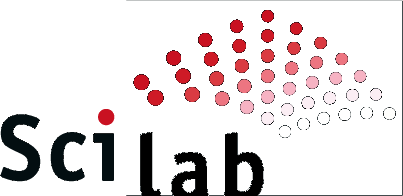
\includegraphics[height=.8cm]{png/logo_scilab}} 
\rotatebox{90}{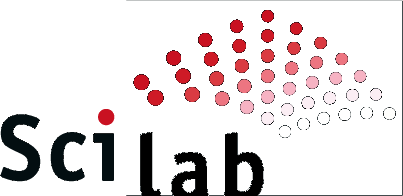
\includegraphics[height=.6cm]{png/logo_scilab}} 
        {\color{violetf}\vrule width 3pt}%
        \hspace{0pt}%must no space.
        \fboxsep=\FrameSep\colorbox{violetc}%
    }%
    \MakeFramed{\hsize #1 \advance\hsize-\width\FrameRestore}%
}%
{\endMakeFramed}%

\newenvironment{pseudo}[1][\hsize]%
{%
    \def\FrameCommand%
    {%
\rotatebox{90}{\textit{\textsf{Pseudo Code}}} 
        {\color{violetf}\vrule width 3pt}%
        \hspace{0pt}%must no space.
        \fboxsep=\FrameSep\colorbox{violetc}%
    }%
    \MakeFramed{\hsize #1 \advance\hsize-\width\FrameRestore}%
}%
{\endMakeFramed}%

\newenvironment{py}[1][\hsize]%
{%
    \def\FrameCommand%
    {%
%\rotatebox{90}{\textit{\textsf{Python}}} 
\rotatebox{90}{
\includegraphics[height=.6cm]{png/logo_python}} 
        {\color{violetf}\vrule width 3pt}%
        \hspace{0pt}%must no space.
        \fboxsep=\FrameSep\colorbox{violetc}%
    }%
    \MakeFramed{\hsize #1 \advance\hsize-\width\FrameRestore}%
}%
{\endMakeFramed}%


\newenvironment{term}[1][\hsize]%
{%
    \def\FrameCommand%
    {%
\rotatebox{90}{\textit{\textsf{Terminal}}} 
        {\color{violetf}\vrule width 3pt}%
        \hspace{0pt}%must no space.
        \fboxsep=\FrameSep\colorbox{violetc}%
    }%
    \MakeFramed{\hsize #1 \advance\hsize-\width\FrameRestore}%
}%
{\endMakeFramed}%


\newenvironment{rem}[1][\hsize]%
{%
    \def\FrameCommand
    {%
\rotatebox{90}{\textit{\textsf{Remarque}}} 
        {\color{bleuf}\vrule width 3pt}%
        \hspace{0pt}%must no space.
        \fboxsep=\FrameSep\colorbox{bleuc}%
    }%
    \MakeFramed{\hsize#1\advance\hsize-\width\FrameRestore}%
}%
{\endMakeFramed}%


\newenvironment{savoir}[1][\hsize]%
{%
    \def\FrameCommand
    {%
\rotatebox{90}{\textit{\textsf{Savoir}}} 
        {\color{bleuf}\vrule width 3pt}%
        \hspace{0pt}%must no space.
        \fboxsep=\FrameSep\colorbox{bleuc}%
    }%
    \MakeFramed{\hsize#1\advance\hsize-\width\FrameRestore}%
}%
{\endMakeFramed}%

\newenvironment{Objectif}[1][\hsize]%
{%
    \def\FrameCommand
    {%
\rotatebox{90}{\textit{\textsf{Objectif}}} 
        {\color{bleuf}\vrule width 3pt}%
        \hspace{0pt}%must no space.
        \fboxsep=\FrameSep\colorbox{bleuc}%
    }%
    \MakeFramed{\hsize#1\advance\hsize-\width\FrameRestore}%
}%
{\endMakeFramed}%

\newenvironment{prob}[1][\hsize]%
{%
    \def\FrameCommand%
    {%
\rotatebox{90}{\textit{\textsf{ Problématique}}} 
        {\color{rougef}\vrule width 3pt}%
        \hspace{0pt}%must no space.
        \fboxsep=\FrameSep\colorbox{rougec}%
    }%
    \MakeFramed{\hsize#1\advance\hsize-\width\FrameRestore}%
}%
{\endMakeFramed}%

\newenvironment{obj}[1][\hsize]%
{%
    \def\FrameCommand%
    {%
\rotatebox{90}{\textit{\textsf{ $\;$}}} 
        {\color{rougef}\vrule width 3pt}%
        \hspace{0pt}%must no space.
        \fboxsep=\FrameSep\colorbox{rougec}%
    }%
    \MakeFramed{\hsize#1\advance\hsize-\width\FrameRestore}%
}%
{\endMakeFramed}%

\newenvironment{defi}[1][\hsize]%
{%
    \def\FrameCommand%
    {%
\rotatebox{90}{\textit{\textsf{Définition\\}}} 
        {\color{bleuf}\vrule width 3pt}%
        \hspace{0pt}%must no space.
        \fboxsep=\FrameSep\colorbox{bleuc}%
    }%
    \MakeFramed{\hsize#1\advance\hsize-\width\FrameRestore}%
}%
{\endMakeFramed}%


\newenvironment{demo}[1][\hsize]%
{%
    \def\FrameCommand%
    {%
\rotatebox{90}{\textit{\textsf{Démonstration\\}}} 
        {\color{bleuf}\vrule width 3pt}%
        \hspace{0pt}%must no space.
        \fboxsep=\FrameSep\colorbox{bleuc}%
    }%
    \MakeFramed{\hsize#1\advance\hsize-\width\FrameRestore}%
}%
{\endMakeFramed}%


\newenvironment{hypo}[1][\hsize]%
{%
    \def\FrameCommand%
    {%
\rotatebox{90}{\textit{\textsf{Hypothèse\\}}} 
        {\color{bleuf}\vrule width 3pt}%
        \hspace{0pt}%must no space.
        \fboxsep=\FrameSep\colorbox{bleuc}%
    }%
    \MakeFramed{\hsize#1\advance\hsize-\width\FrameRestore}%
}%
{\endMakeFramed}%


\newenvironment{prop}[1][\hsize]%
{%
    \def\FrameCommand%
    {%
\rotatebox{90}{\textit{\textsf{Propriété\\}}} 
        {\color{bleuf}\vrule width 3pt}%
        \hspace{0pt}%must no space.
        \fboxsep=\FrameSep\colorbox{bleuc}%
    }%
    \MakeFramed{\hsize#1\advance\hsize-\width\FrameRestore}%
}%
{\endMakeFramed}%

\newenvironment{props}[1][\hsize]%
{%
    \def\FrameCommand%
    {%
\rotatebox{90}{\textit{\textsf{Propriétés\\}}} 
        {\color{bleuf}\vrule width 3pt}%
        \hspace{0pt}%must no space.
        \fboxsep=\FrameSep\colorbox{bleuc}%
    }%
    \MakeFramed{\hsize#1\advance\hsize-\width\FrameRestore}%
}%
{\endMakeFramed}%

\newenvironment{exemple}[1][\hsize]%
{%
    \def\FrameCommand%
    {%
\rotatebox{90}{\textit{\textsf{Exemple\\}}} 
        {\color{vertf}\vrule width 3pt}%
        \hspace{0pt}%must no space.
        \fboxsep=\FrameSep\colorbox{vertc}%
    }%
    \MakeFramed{\hsize#1\advance\hsize-\width\FrameRestore}%
}%
{\endMakeFramed}%

\newenvironment{exercice}[1][\hsize]%
{%
    \def\FrameCommand%
    {%
\rotatebox{90}{\textit{\textsf{Exercice\\}}} 
        {\color{vertf}\vrule width 3pt}%
        \hspace{0pt}%must no space.
        \fboxsep=\FrameSep\colorbox{vertc}%
    }%
    \MakeFramed{\hsize#1\advance\hsize-\width\FrameRestore}%
}%
{\endMakeFramed}%

\newenvironment{Support}[1][\hsize]%
{%
    \def\FrameCommand%
    {%
\rotatebox{90}{\textit{\textsf{Support de cours\\}}} 
        {\color{vertf}\vrule width 3pt}%
        \hspace{0pt}%must no space.
        \fboxsep=\FrameSep\colorbox{jaunec}%
    }%
    \MakeFramed{\hsize#1\advance\hsize-\width\FrameRestore}%
}%
{\endMakeFramed}%

\newenvironment{resultat}[1][\hsize]%
{%
    \def\FrameCommand%
    {%
\rotatebox{90}{\textit{\textsf{Résultat\\}}} 
        {\color{rougef}\vrule width 3pt}%
        \hspace{0pt}%must no space.
        \fboxsep=\FrameSep\colorbox{rougec}%
    }%
    \MakeFramed{\hsize#1\advance\hsize-\width\FrameRestore}%
}%
{\endMakeFramed}%

\newenvironment{methode}[1][\hsize]%
{%
    \def\FrameCommand%
    {%
\rotatebox{90}{\textit{\textsf{Méthode\\}}} 
        {\color{rougef}\vrule width 3pt}%
        \hspace{0pt}%must no space.
        \fboxsep=\FrameSep\colorbox{rougec}%
    }%
    \MakeFramed{\hsize#1\advance\hsize-\width\FrameRestore}%
}%
{\endMakeFramed}%

\newenvironment{theo}[1][\hsize]%
{%
    \def\FrameCommand%
    {%
\rotatebox{90}{\textit{\textsf{Théorème\\}}} 
        {\color{rougef}\vrule width 3pt}%
        \hspace{0pt}%must no space.
        \fboxsep=\FrameSep\colorbox{rougec}%
    }%
    \MakeFramed{\hsize#1\advance\hsize-\width\FrameRestore}%
}%
{\endMakeFramed}%

\newenvironment{warn}[1][\hsize]%
{%
    \def\FrameCommand%
    {%
\rotatebox{90}{\textit{\textsf{Attention\\}}} 
        {\color{rougef}\vrule width 3pt}%
        \hspace{0pt}%must no space.
        \fboxsep=\FrameSep\colorbox{rougec}%
    }%
    \MakeFramed{\hsize#1\advance\hsize-\width\FrameRestore}%
}%
{\endMakeFramed}%
 \usepackage{cancel}

%Si le boolen xp est vrai : compilation pour xabi
%Sinon compilation Damien
\newboolean{xp}
\setboolean{xp}{true}

\newboolean{prof}
\setboolean{prof}{true}

\usepackage[%
    pdftitle={CI 09 :  - Ch 02 : PFS},
    pdfauthor={Xavier Pessoles},
    colorlinks=true,
    linkcolor=blue,
    citecolor=magenta]{hyperref}


\def\discipline{Sciences Industrielles de l'Ingénieur}
\def\xxtitre{\ifthenelse{\boolean{xp}}{
CI 9 : Étude des mécanismes complexes}{}}

\def\xxsoustitre{\ifthenelse{\boolean{xp}}{
Chapitre 1 -- Introduction aux chaînes de solides}{
Partie  -- }}

\def\xxauteur{\ifthenelse{\boolean{xp}}{
Xavier \textsc{Pessoles}}{}}

\def\xxpied{\ifthenelse{\boolean{xp}}{
CI 9 : Étude des mécanismes complexes\\
Ch. 1 : Intro. aux chaînes de solides -- Cours}{
\xxtitre}}

\def\xxcathegorie{\ifthenelse{\boolean{xp}}{
2013 -- 2014 \\
Xavier \textsc{Pessoles}}{}}





%---------------------------------------------------------------------------


\begin{document}

\ifthenelse{\boolean{xp}}{
\sloppy
\hyphenpenalty 10000


%------------- En tetes et Pieds de Pages ------------

\pagestyle{fancy}
\renewcommand{\headrulewidth}{0pt}
\fancyhead{}
\fancyhead[L]{%
\noindent\begin{minipage}[c]{2.6cm}%

\includegraphics[width=2cm]{png/logo_ptsi.png}%
\end{minipage}}


\fancyhead[C]{\rule{12cm}{.5pt}}


\fancyhead[R]{%
\noindent\begin{minipage}[c]{3cm}
\begin{flushright}
\footnotesize{\textit{\textsf{\discipline}}}%
\end{flushright}
\end{minipage}
}



\fancyhead[C]{\rule{12cm}{.5pt}}

\renewcommand{\footrulewidth}{0.2pt}

\fancyfoot[C]{\footnotesize{\bfseries \thepage}}
\fancyfoot[L]{%
\begin{minipage}[c]{.2\linewidth}
\noindent\footnotesize{{\xxauteur}}
\end{minipage}
}

%\ifthenelse{\boolean{prof}}}

\begin{center}
 \huge\textsc{\xxtitre}
\end{center}

\begin{center}
 \LARGE\textsc{\xxsoustitre}
\end{center}

\vspace{.5cm}
}{\ifthenelse{\boolean{xp}}{
\usepackage[%
    pdftitle={OS et Environnement de développement},
    pdfauthor={Xavier Pessoles},
    colorlinks=true,
    linkcolor=blue,
    citecolor=magenta]{hyperref}}{
\usepackage[%
    pdftitle={OS et Environnement de développement},
    pdfauthor={Damien Iceta},
    colorlinks=true,
    linkcolor=blue,
    citecolor=magenta]{hyperref}}

\usepackage{pifont}
\usepackage{lastpage}

% \makeatletter \let\ps@plain\ps@empty \makeatother
%% DEBUT DU DOCUMENT
%% =================
\sloppy
\hyphenpenalty 10000

\newcommand{\Pointilles}[1][3]{%
\multido{}{#1}{\makebox[\linewidth]{\dotfill}\\[\parskip]
}}


\colorlet{shadecolor}{orange!15}

\newtheorem{theorem}{Theorem}


\begin{document}


\newboolean{prof}
\setboolean{prof}{true}
%------------- En tetes et Pieds de Pages ------------


\pagestyle{fancy}
%\renewcommand{\headrulewidth}{0}
\renewcommand{\headrulewidth}{0.2pt} %pour mettre le trait en haut

\fancyhead{}
\fancyhead[L]{
\footnotesize{{{\xxtitre}}}%
%\noindent\noindent\begin{minipage}[c]{2.6cm}
%\includegraphics[width=2.5cm]{png/logo.png}%
%\end{minipage}
}

%\fancyhead[C]{\rule{12cm}{.5pt}}  %pour mettre le petit trait en haut


\fancyhead[R]{%
\noindent\begin{minipage}[c]{3cm}
\begin{flushright}
\footnotesize{{{\xxcathegorie}}}%
\end{flushright}
\end{minipage}
}

\renewcommand{\footrulewidth}{0.2pt}

\fancyfoot[C]{\footnotesize{}}
\fancyfoot[L]{%
\begin{minipage}[l]{.2\linewidth}
\noindent\footnotesize{{\xxauteur}}
\end{minipage}
\begin{minipage}[c]{.15\linewidth}
%
\includegraphics[width=2cm]{png/logoCC.png}
\end{minipage}}

\ifthenelse{\boolean{prof}}{%
\fancyfoot[R]{\footnotesize{Page \thepage\   sur  \pageref{LastPage}}}}

\begin{center}
 \huge\textsc{\xxtitre}
\end{center}

\begin{center}
 \LARGE\textsc{\xxsoustitre}
\end{center}

\vspace{.5cm}}



\begin{center}
\begin{tabular}{cccc}
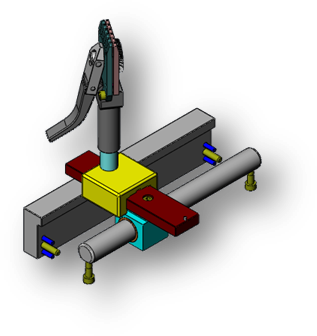
\includegraphics[height=3cm]{images/ex1} &
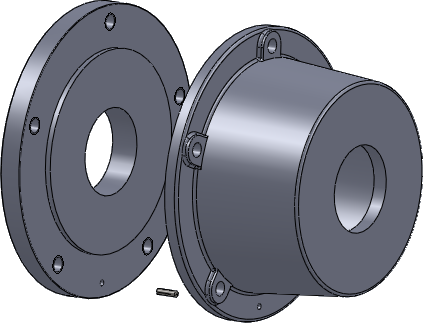
\includegraphics[height=3cm]{images/ex2} &
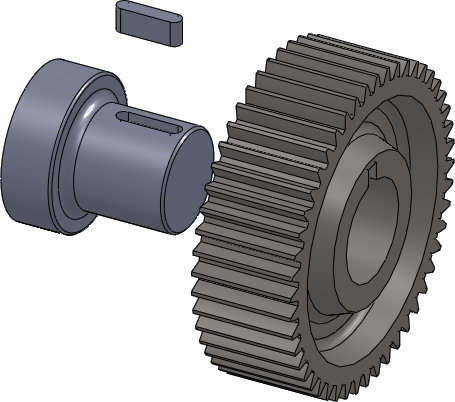
\includegraphics[height=3cm]{images/ex3} &
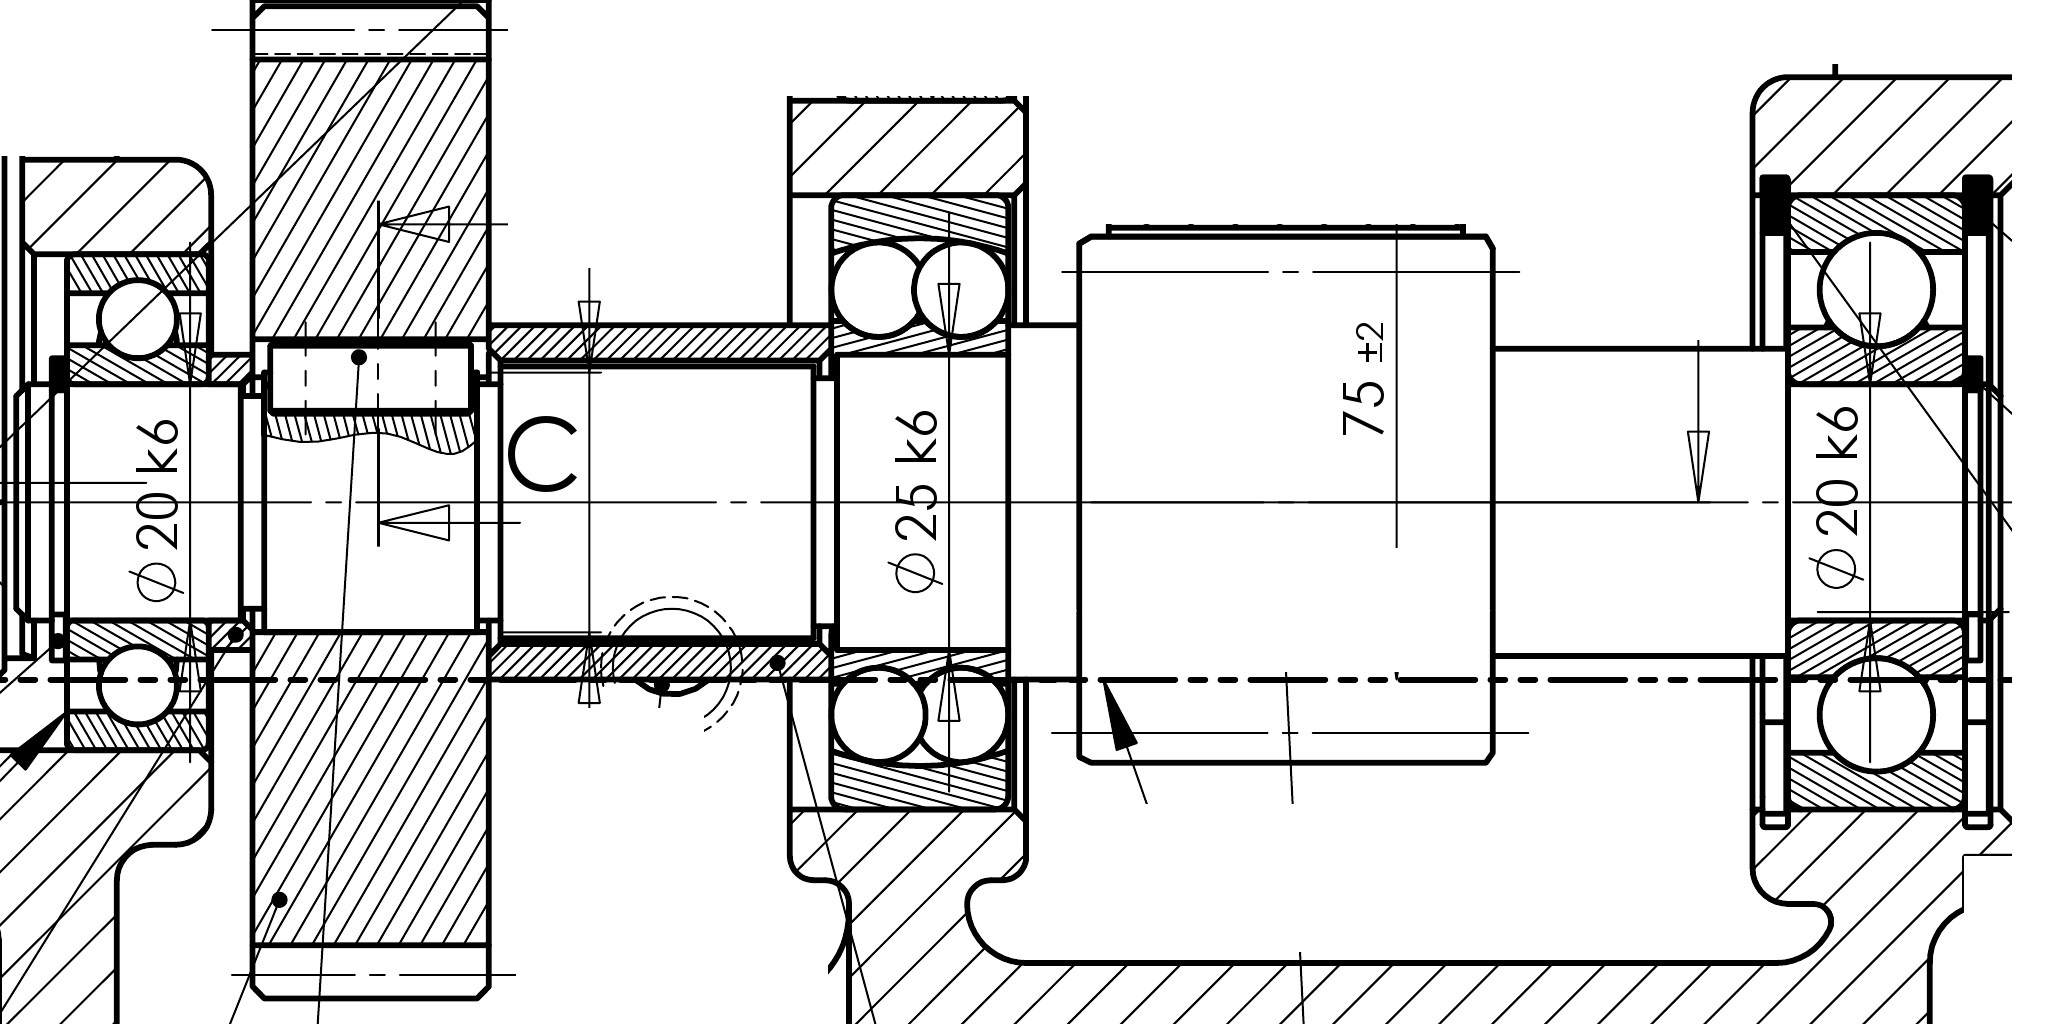
\includegraphics[height=3cm]{images/ex4} \\
\textit{Pince de la cordeuse} & 
\textit{Montage de carters} &
\textit{Montage d'une poulie} &
\textit{Montage de roulement}\\
\end{tabular}
\end{center}

Lors de la résolution d'un problème de mécanique, plusieurs problèmes peuvent parfois se poser. Par exemple, en cinématique, dans le cas d'un calcul de loi entrée/sortie, des liaisons pourraient parfois être associées afin de simplifier les calculs. D'autre part en statique, il est souvent pertinent de s'interroger sur la faisabilité du problème. En effet, dans certain cas, toutes les inconnues ne peuvent pas être déterminées.


\begin{prob}
\textsc{Problématique :}
\begin{itemize}
\item Comment associer des liaisons afin de simplifier les calculs de cinématique ?
\item Comment prévoir si un problème de statique peut être résolu ou non ?
\end{itemize}
\end{prob}

\begin{savoir}
\textsc{Savoirs :}
\begin{itemize}
\item Mod-C14.1 : Liaison cinématiquement équivalente
\item Mod-C14.2 : Mobilité d’une chaîne ouverte
\item Mod-C14.3 : Hyperstatisme et mobilité d’une chaîne fermée
\begin{itemize}
\item Mod-C14-S3 : Déterminer la liaison cinématiquement équivalente à une association de liaisons
\item Mod-C14-S4 : Déterminer les mobilités d’un mécanisme
\item Mod-C14-S5 : Déterminer le degré d’hyperstaticité d’un mécanisme
\item Mod-C14-S6 : Identifier les conséquences géométriques de l’hyperstaticité.
\end{itemize}
\end{itemize}
\end{savoir}

\setlength{\parskip}{0ex plus 0.2ex minus 0ex}
 \renewcommand{\contentsname}{}
 \renewcommand{\baselinestretch}{1}

\tableofcontents

 \renewcommand{\baselinestretch}{1.2}
\setlength{\parskip}{2ex plus 0.5ex minus 0.2ex}

% \vspace{1cm}
\textit{Ce document est en évolution permanente. Merci de signaler toutes
erreurs ou coquilles.}

\section{Détermination des liaisons équivalentes}
\subsection{Rappels}
\begin{defi}

\textbf{Structure des chaînes}

\begin{center} 
\begin{tabular}{ccc}
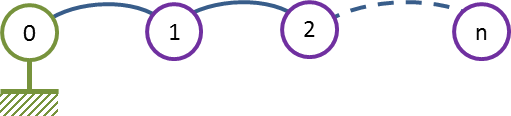
\includegraphics[height=1.5cm]{images/def_co} &
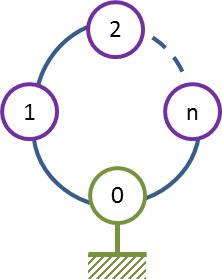
\includegraphics[height=3cm]{images/def_cf} &
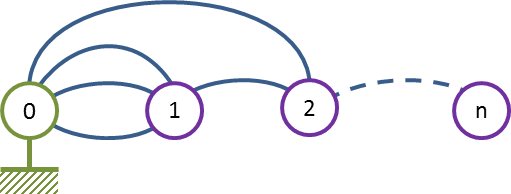
\includegraphics[height=2cm]{images/def_cc} \\
\textbf{Chaîne ouverte}&
\textbf{Chaîne fermée}&
\textbf{Chaîne complexe}
\end{tabular}
\end{center}
\end{defi}

\begin{defi}

\textbf{Décomposition du torseur cinématique}

Soient $n$ solides en chaîne ouverte. On a :
$$
\torseurcin{V}{1}{n} = \torseurcin{V}{1}{2} + \torseurcin{V}{2}{3} + ... + \torseurcin{V}{n-1}{n}
=\sum\limits_{i=1}^{n-1} \torseurcin{V}{n}{n+1}
$$
En utilisant le vecteur instantané de rotation et le vecteur vitesse exprimé en un point $P$, on a donc : 
$$
\left\{
\begin{array}{l}
\vecto{1}{n} = \vecto{1}{2} + \vecto{2}{3} + ... +\vecto{n-1}{n} \\
\vectv{P}{1}{n} = \vectv{P}{1}{2} +\vectv{P}{2}{3} + ... + \vectv{P}{n-1}{n}
\end{array}
\right.
$$
\end{defi}


\begin{defi}

\textbf{Principe fondamental de la statique}

Soient $n$ solides liés au solide 1. En isolant 1, d'après le principe fondamental de la statique appliqué au point 1, on a : 
$$
\torseurstat{T}{2}{1} + \torseurstat{T}{3}{1} + ... + \torseurstat{T}{n}{1}
=\{0\}
$$
En utilisant le théorème de la résultante statique et le théorème du moment statique au point $P$, on a donc : 
$$
\left\{
\begin{array}{l}
\vectf{2}{1} +\vectf{3}{1} +  ... +\vectf{n}{1} = \vect{0} \\
\vectm{P}{2}{1} + \vectm{P}{3}{1} + ... + \vectm{P}{n}{1} = \vect{0}
\end{array}
\right.
$$
\end{defi}

\subsection{Méthodes}

\begin{methode}
\textbf{Liaisons en séries}

\begin{center}
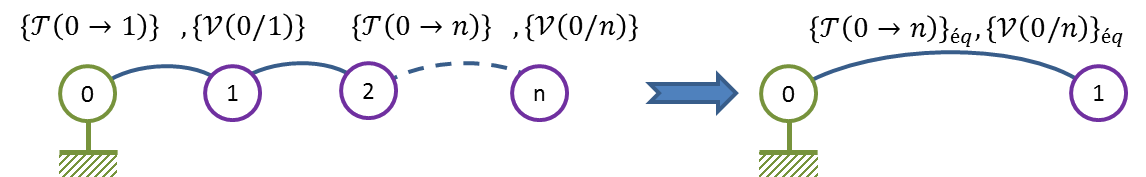
\includegraphics[width=.6\textwidth]{images/serie}
\end{center}

\begin{minipage}[t]{.47\linewidth}
\noindent\colorbox{rougef}{\makebox[\textwidth][l]{%
\textbf{\textsf{\textcolor{white}{Méthode statique}}}
}}
\begin{enumerate}
\item On pose : 
$$
\{\mathcal{T}_{eq}\}=\torseurcol{X_{eq}}{Y_{eq}}{Z_{eq}}{L_{eq}}{M_{eq}}{N_{eq}}{P,\mathcal{R}}
$$
\item Écrire les torseurs \textbf{statiques} de chacune des liaisons.
\item Déplacer les torseurs au même point.
\item On applique le PFS à chacun des solides.
%: $$
%\{\mathcal{T}_{eq}\}=\torseurstat{T}{\overline{i}}{i}
%=...
%=\torseurstat{T}{n-1}{n}
%$$
\item Ainsi, s'il y a $n$ solides (hors bâti), le PFS permet donc d'écrire $n$ équations.
%\item Suivant les composantes de $\{\mathcal{T}_{eq}\}$ on peut donc l'associer à une liaison usuelle, ou non.
\end{enumerate}
\end{minipage}\hfill
\begin{minipage}[t]{.47\linewidth}
\noindent\colorbox{rougef}{\makebox[\textwidth][l]{%
\textbf{\textsf{\textcolor{white}{Méthode cinématique}}}
}}
\begin{enumerate}
\item On pose : 
$$
\{\mathcal{V}_{eq}\}=\torseurcol{\alpha_{eq}}{\beta_{eq}}{\gamma_{eq}}{u_{eq}}{v_{eq}}{w_{eq}}{P,\mathcal{R}}
$$
\item Écrire les torseurs \textbf{cinématiques} de chacune des liaisons.
\item Déplacer les torseurs au même point.
\item D'après la composition du torseur cinématique, on a alors : 
$$
\{\mathcal{V}_{eq} \}=\torseurcin{V}{0}{1}+...
+\torseurstat{V}{n-1}{n}
$$
\item Suivant les composantes de $\{\mathcal{V}_{eq}\}$ on peut donc l'associer à une liaison usuelle, ou non.
\end{enumerate}
\end{minipage}
\end{methode}



\begin{methode}
\textbf{Liaisons en parallèles}

\begin{center}
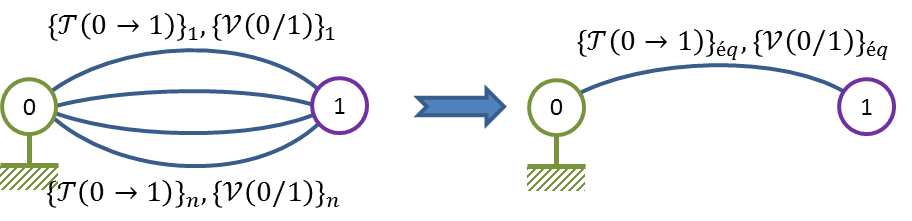
\includegraphics[width=.5\textwidth]{images/parallele}
\end{center}

\begin{minipage}[t]{.47\linewidth}
\noindent\colorbox{rougef}{\makebox[\textwidth][l]{%
\textbf{\textsf{\textcolor{white}{Méthode statique}}}
}}
\begin{enumerate}
\item On pose : 
$$
\{\mathcal{T}_{eq}\}=\torseurcol{X_{eq}}{Y_{eq}}{Z_{eq}}{L_{eq}}{M_{eq}}{N_{eq}}{P,\mathcal{R}}
$$
\item Écrire les torseurs \textbf{statiques} de chacune des liaisons.
\item Déplacer les torseurs au même point.
\item On a alors : $$
\{\mathcal{T}_{eq}\}=\torseurstat{T}{0}{1}
+...
+\torseurstat{T}{n-1}{n}
$$
\item Suivant les composantes de $\{\mathcal{T}_{eq}\}$ on peut donc l'associer à une liaison usuelle, ou non.
\end{enumerate}
\end{minipage}\hfill
\begin{minipage}[t]{.47\linewidth}
\noindent\colorbox{rougef}{\makebox[\textwidth][l]{%
\textbf{\textsf{\textcolor{white}{Méthode cinématique}}}
}}
\begin{enumerate}
\item On pose : 
$$
\{\mathcal{V}_{eq}\}=\torseurcol{\alpha_{eq}}{\beta_{eq}}{\gamma_{eq}}{u_{eq}}{v_{eq}}{w_{eq}}{P,\mathcal{R}}
$$
\item Écrire les torseurs \textbf{cinématiques} de chacune des liaisons.
\item Déplacer les torseurs au même point.
\item On a alors : 
$$
\{\mathcal{V}_{eq} \}=\torseurcin{V}{0}{1}=...
=\torseurcin{V}{n-1}{n}
$$
\item Suivant les composantes de $\{\mathcal{V}_{eq}\}$ on peut donc l'associer à une liaison usuelle, ou non.
\end{enumerate}
\end{minipage}
\end{methode}


\begin{rem}
Il est souvent plus facile de faire une somme de torseurs plutôt que de résoudre un système de $n$ équations. Pour calculer des liaisons équivalente, on utilisera donc, de préférence : 
\begin{itemize}
\item \textbf{pour les liaisons en séries}, la méthode cinématique;
\item \textbf{pour les en parallèles}, la méthode statique.
\end{itemize}
\end{rem}




\subsection{Chaînes ouvertes}

\begin{exemple}
\begin{center}
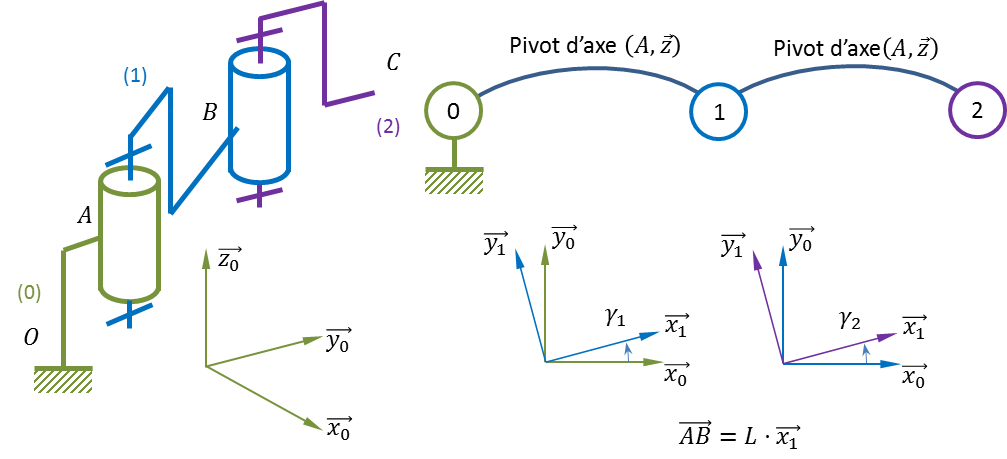
\includegraphics[width=.8\textwidth]{images/co}
\end{center}

\end{exemple}

\noindent\colorbox{grisf}{\makebox[\textwidth][l]{%
\textbf{\textsf{Méthode 1 -- Composition du torseur cinématique}}
}}

Torseur cinématique de la liaison pivot en $A$ entre 0 et 1 :
$$
\torseurcin{V}{1}{0}=
\torseurl{%
\vecto{1}{0}=\dot{\gamma}_1\vect{z_0}
}{%
\vectv{A}{1}{0}=\vect{0}
}{%
A}
$$

Torseur cinématique de la liaison pivot en $B$ puis en $A$ entre 2 et 1 :
$$
\torseurcin{V}{2}{1}=
\torseurl{%
\vecto{2}{1}=\dot{\gamma}_2\vect{z_0}
}{%
\vectv{B}{2}{1}=\vect{0}
}{%
B}\\
=
\torseurl{%
\vecto{2}{1}=\dot{\gamma}_2\vect{z_0}
}{%
\vectv{A}{2}{1}=-L\dot{\gamma}_2\vect{y_1}
}{%
A}
$$

Par composition du torseur cinématique, on a :
$$
\torseurcin{V}{2}{1}+\torseurcin{V}{1}{0}=\torseurcin{V}{2}{0}
$$

$$
\torseurcin{V}{2}{0}=
\torseurl{%
\vecto{2}{0}=\left( \dot{\gamma}_1+\dot{\gamma}_2\right)\vect{z_0}
}{%
\vectv{A}{2}{0}=-L\dot{\gamma}_2\vect{y_1}
}{%
A}\\
=
\torseurl{%
\vecto{2}{0}=\left( \dot{\gamma}_1+\dot{\gamma}_2 \right)\vect{z_0}
}{%
\vectv{A}{2}{0}=-L\dot{\gamma}_2\left( \cos{\gamma}_1 \vect{y_0}-\sin{\gamma}_1\vect{x_0}\right)
}{%
A}
=
\torseurcol{0}{0}{\dot{\gamma}_{eq}}{\dot{u}_{eq}}{\dot{v}_{eq}}{0}{A}
$$

Cette liaison permet donc deux translations suivant $\vect{x_0}$ et $\vect{y_0}$ et une rotation autour de $\vect{z_0}$. La liaison équivalente à ces deux liaisons pivot en série est donc une liaison appui-plan. 


\noindent\colorbox{grisf}{\makebox[\textwidth][l]{%
\textbf{\textsf{Méthode 2 -- Utilisation des torseurs statiques}}
}}
Torseur statique de la liaison pivot en $A$ entre 0 et 1 :
$$
\torseurstat{T}{0}{1}=
\torseurcol{X_{01}}{Y_{01}}{Z_{01}}{L_{01}}{M_{01}}{0}{A,\mathcal{R}_0}
$$

Torseur statique de la liaison pivot en $B$ puis en $A$ entre 2 et 1 :
$$
\torseurstat{T}{2}{1}=
\torseurcol{X_{21}}{Y_{21}}{Z_{21}}{L_{21}}{M_{21}}{0}{B,\mathcal{R}_0}\\
=
\torseurcol{X_{21}}{Y_{21}}{Z_{21}}{L_{21}+L\sin\gamma_1 Z_{21}}{M_{21}-L\cos\gamma_1 Z_{21}}{L\cos\gamma_1 Y_{21}-L\sin\gamma_1 X_{21}}{A,\mathcal{R}_0}\\
$$

D'après le PFS appliqué au solide 1, 
$\torseurstat{T}{2}{1}+\torseurstat{T}{0}{1}=\{0\}$.
Le torseur équivalent à la liaison entre 0 et 2 est donc tel que :
$$
\torseurstat{T}{1}{2}=\torseurstat{T}{0}{1}=\{\mathcal{T}_{eq}\}
$$

$$
\left\{
\begin{array}{l}
X_{12}=X_{01}=X_{eq}\\
Y_{12}=Y_{01}=Y_{eq}\\
Z_{12}=Z_{01}=Z_{eq}\\
L_{12}+L\sin\theta Z_{12}=L_{01}=L_{eq}\\
M_{12}+L\cos\theta Z_{12}=M_{01}=M_{eq}\\
L\cos\theta Y_{12}-L\sin\theta X_{12}=0=N_{eq}
\end{array}
\right.
\Longleftrightarrow
\left\{
\begin{array}{l}
X_{12}=X_{01}=X_{eq}\\
Y_{12}=Y_{01}=Y_{eq}\\
Z_{eq}\neq 0\\
L_{eq}\neq 0\\
M_{eq}\neq 0\\
N_{eq}=0 \\
Y_{12}\cos\theta- X_{12}\sin\theta=0
\end{array}
\right.
$$


\textit{Nécessairement $X_{12}=0$ et $Y_{12}=0$.}

La liaison équivalente a donc pour torseur la forme suivante :
$$
\{\mathcal{T}_{eq}\}=
\torseurcol{0}{0}{Z_{eq}}{L_{eq}}{M_{eq}}{0}{A,\mathcal{R}_1}
$$


\subsection{Chaînes fermées}
\begin{exemple}
\begin{center}
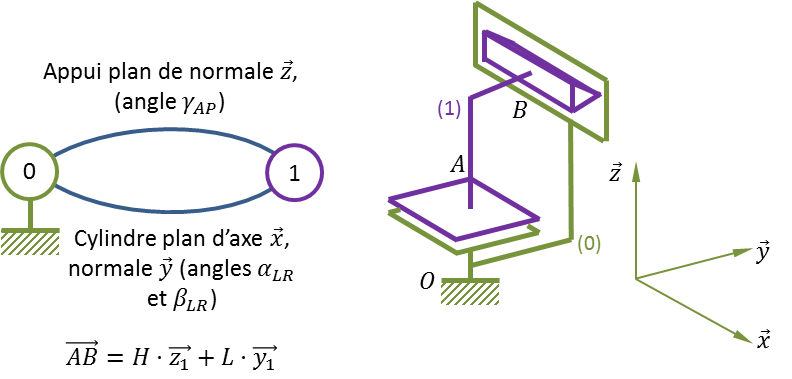
\includegraphics[width=.6\textwidth]{images/cf}
\end{center}
\end{exemple}

\noindent\colorbox{grisf}{\makebox[\textwidth][l]{%
\textbf{\textsf{Méthode 1 -- Utilisation du torseur cinématique}}
}}


Torseur cinématique de la liaison appui-plan en $A$ entre 0 et 1 :
$$
\torseurcin{V}{1}{0}_{AP}=
\torseurl{%
\vecto{1}{0}_{AP}=\dot{\gamma}_{AP}\vect{z_1}
}{%
\vectv{A}{1}{0}_{AP}=\dot{u}_{AP}\vect{x_1}+\dot{v}_{AP}\vect{y_1}
}{%
A}
$$

Torseur cinématique de la liaison linéaire rectiligne en $B$ puis en $A$ entre 1 et 0 :
\begin{eqnarray*}
\torseurcin{V}{1}{0}_{LR}&=&
\torseurl{%
\vecto{1}{0}_{LR}=\dot{\alpha}_{LR}\vect{x_1}+\dot{\beta}_{LR}\vect{y_1}
}{%
\vectv{B}{1}{0}_{LR}=\dot{u}_{LR}\vect{x_1}+\dot{w}_{LR}\vect{z_1}
}{%
B}\\
&=&
\torseurl{%
\vecto{1}{0}_{LR}=\dot{\alpha}_{LR}\vect{x_1}+\dot{\beta}_{LR}\vect{y_1}
}{%
\vectv{A}{1}{0}_{LR}=\left(\dot{u}_{LR}-H\dot{\beta}_{LR} \right)\vect{x_1}+H\dot{\alpha}_{LR}\vect{y_1}+\left(\dot{w}_{LR}+L\dot{\alpha}_{LR} \right)\vect{z_1}
}{%
A}
\end{eqnarray*}

Les deux liaisons étant en parallèles, il est nécessaire qu'elles permettent les mêmes mobilités. En conséquence, on doit avoir :
$$
\torseurcin{V}{1}{0}_{LR} = \torseurcin{V}{1}{0}_{AP}
$$

En conséquence : 

\noindent\begin{minipage}[c]{.45\linewidth}
$$
\left\{
\begin{array}{l}
\dot{\alpha}_{LR}=0 \\
\dot{\beta}_{LR}=0 \\
0=\dot{\gamma_{AP}} \\
\dot{u}_{LR}-H\dot{\beta} =\dot{u}_{AP} \\
H\dot{\alpha}_{LR}= \dot{v}_{AP} \\
\dot{w}_{LR}+L\dot{\alpha} _{LR}= 0
\end{array}
\right.
\Longleftrightarrow
\left\{
\begin{array}{l}
\dot{\alpha_{LR}}=0 \\
\dot{\beta_{LR}}=0 \\
\dot{\gamma_{AP}}=0 \\
\dot{u_{LR}} =\dot{u_{AP}} \\
 \dot{v_{AP}} = 0\\
\dot{w_{LR}} = 0
\end{array}
\right.
$$
\end{minipage}\hfill
\begin{minipage}[c]{.5\linewidth}
\begin{center}
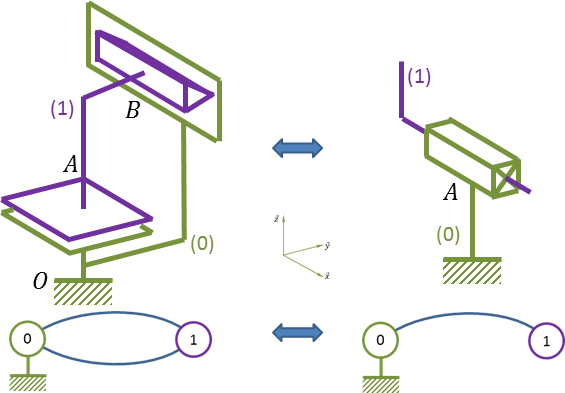
\includegraphics[width=\textwidth]{images/cf_eq}
\end{center}
\end{minipage}

Au final, 
$$
\{\mathcal{V}_{eq}\}=
\torseurcol{0}{0}{0}{\dot{u}}{0}{0}{A}
$$

\vspace{.25cm}

La seule composante non nulle du torseur cinématique est donc la vitesse de déplacement suivant $\vect{x_1}$. La liaison est donc une liaison glissière d'axe $\vect{x_1}$


\noindent\colorbox{grisf}{\makebox[\textwidth][l]{%
\textbf{\textsf{Méthode 2 -- Utilisation du torseur statique}}
}}

Torseur statique de la liaison appui-plan en $A$ entre 0 et 1 :
$$
\torseurstat{T}{1}{0}_{AP}=
\torseurcol{0}{0}{Z_{01,AP}}{L_{01,AP}}{M_{01,AP}}{0}{A,\mathcal{R}_1}
$$

Torseur statique de la liaison linéaire rectiligne en $B$ puis en $A$ entre 1 et 0 :
$$
\torseurstat{T}{1}{0}_{LR}=
\torseurcol{0}{Y_{01,LR}}{0}{0}{0}{N_{01,LR}}{B,\mathcal{R}_1}
=
\torseurcol{0}{Y_{01,LR}}{0}{-HY_{01,LR}}{0}{N_{01,LR}}{A,\mathcal{R}_1}
$$


En appliquant le PFS au solide 1 au point A, on a donc :
$$
\torseurstat{T}{0}{1}_{AP}+\torseurstat{T}{0}{1}_{LR}=\{\mathcal{T}_{eq}\}
$$

$$
\left\{
\begin{array}{l}
0+0 = X \\
0+Y_{01,LR}=Y\\
Z_{01,AP}+0=Z\\
L_{01,AP}-HY_{01,LR}=L\\
M_{01,AP}+0=M\\
0+N_{01,LR}=N
\end{array}
\right.
\Longleftrightarrow
\left\{
\begin{array}{l}
X = 0 \\
Y=Y_{01,LR}\\
Z=Z_{01,AP}\\
L=L_{01,AP}-HY_{01,LR}\\
M=M_{01,AP}\\
N=0+N_{01,LR}
\end{array}
\right.
\Longleftrightarrow
\{\mathcal{T}_{eq}\} =
\torseurcol{0}{Y}{Z}{L}{M}{N}{A,\mathcal{R}_1}
$$

Les deux liaisons en parallèles sont donc équivalentes à une liaison glissière d'axe $\vect{x_1}$.
\subsection{Chaînes complexes}
\begin{exemple}
\begin{center}
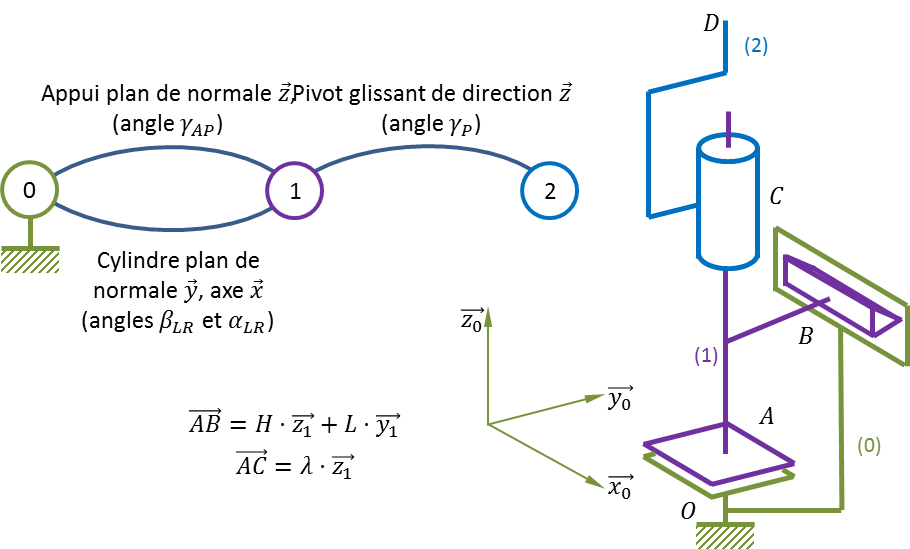
\includegraphics[width=.8\textwidth]{images/cc}
\end{center}
\end{exemple}

Dans ce schéma, on identifie d'abord que les liaisons entre 0 et 1 sont en parallèles.
On a déjà vu que la liaison équivalente (appui-plan et linéaire rectiligne) était une liaison glissière d'axe $\vect{x}$. La chaîne complexe précédente est alors équivalente à la suivante : 

\noindent\begin{minipage}[c]{.45\linewidth}
\begin{center}
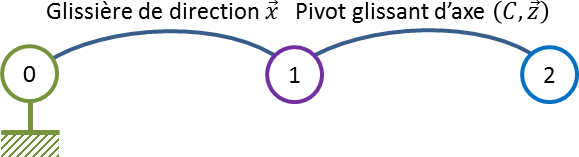
\includegraphics[width=.95\textwidth]{images/cc_2}
\end{center}
\end{minipage}\hfill
\begin{minipage}[c]{.5\linewidth}
Avec $\torseurstat{T}{1}{0}=\torseurcol{0}{Y_{10}}{Z_{10}}{L_{10}}{M_{10}}{N_{10}}{A,\mathcal{R}_1}$ ou $\torseurcin{V}{1}{0}=\torseurcol{0}{0}{0}{\dot{u}_{10}}{0}{0}{A,\mathcal{R}_1}$.
\end{minipage}

\noindent
\colorbox{grisf}{\makebox[\textwidth][l]{%
\textbf{\textsf{Méthode 1 -- Utilisation du torseur cinématique}}
}}

Torseur cinématique de la liaison glissière en $A$ entre 1 et 0 : 
$\torseurcin{V}{1}{0}=\torseurcol{0}{0}{0}{\dot{u}_{10}}{0}{0}{A,\mathcal{R}_1}$

Torseur cinématique de la liaison pivot glissant en $A$ entre 2 et 1 :
$\torseurcin{V}{2}{1}=\torseurcol{0}{0}{\dot{\gamma}_{21}}{0}{0}{\dot{w}_{21}}{A,\mathcal{R}_1}
$

La liaison équivalente à la chaîne cinématique est donc la suivante : 
$$\{\mathcal{V}_{eq}\}=\torseurcin{V}{2}{0}=\torseurcin{V}{2}{1}+\torseurcin{V}{1}{0}
=\torseurcol{0}{0}{\dot{\gamma}_{21}}{\dot{u_{10}}}{0}{\dot{w}_{21}}{A,\mathcal{R}_1}
$$

Cette liaison permet donc trois degrés de liberté : deux translations suivant $\vect{x}$ et $\vect{z}$ et une rotation autour de $\vect{z}$. Cette liaison équivalente n'est pas associable à une liaison usuelle. 

\noindent\colorbox{grisf}{\makebox[\textwidth][l]{%
\textbf{\textsf{Méthode 2 -- Utilisation du torseur statique}}
}}

Torseur statique de la liaison glissière en $A$ entre 1 et 0 : 
$\torseurstat{T}{1}{0}=\torseurcol{0}{Y_{10}}{Z_{10}}{L_{10}}{M_{10}}{N_{10}}{A,\mathcal{R}_1}$

Torseur statique de la liaison pivot glissant en $A$ entre 2 et 1 :
$\torseurstat{T}{2}{1}=\torseurcol{X_{20}}{Y_{20}}{0}{L_{20}}{M_{20}}{0}{A,\mathcal{R}_1}
$

La liaison équivalente à la chaîne cinématique est donc la suivante : 
$$
\{\mathcal{T}_{eq}\}=\torseurstat{T}{2}{1}+\torseurstat{T}{1}{0}
\Longleftrightarrow
\left\{
\begin{array}{l}
0=X_{20}\\
Y_{10}=Y_{20}\\
Z_{10}=0\\
L_{10}=L_{20}\\
M_{10}=M_{20}\\
N_{10}=0
\end{array}
\right.
\{\mathcal{T}_{eq}\}=
\torseurcol{0}{Y_{20}}{0}{L_{20}}{M_{20}}{0}{A,\mathcal{R}_1}
$$

Cette liaison a donc trois degrés de liaison : une translation suivant $\vect{y}$ et deux rotations autour de $\vect{x}$ et $\vect{y}$. Cette liaison équivalente n'est pas associable à une liaison usuelle. 


\section{Notions d'hyperstatismes}

\begin{defi}
\textbf{Hyperstatisme}
Un système est dit hyperstatique lorsque l'application du PFS ne permet pas de calculer toutes les inconnues d'effort dans les liaisons. 

On parle alors de degré d'hyperstatisme, noté $h$. Il correspond au nombre d'inconnues qu'il faudrait imposer pour pouvoir calculer les inconnues restantes. 

\begin{itemize}
\item Si $h>0$ : le mécanisme est dit hyperstatique (trop d'inconnues de liaisons ou trop de degré de liberté supprimés), le fonctionnement correct du mécanisme nécessitera $h$ conditions géométriques.
\item Si $h=0$ : le mécanisme est dit isostatique. 
\item Si $h<0$ : le mécanisme est dit hypostatique (trop de degrés de liberté, pas de transmission possible de la puissance ou dysfonctionnement).
\end{itemize}

\end{defi}

\subsection{Cas d'une chaîne fermée}


\begin{exemple}
\begin{center}
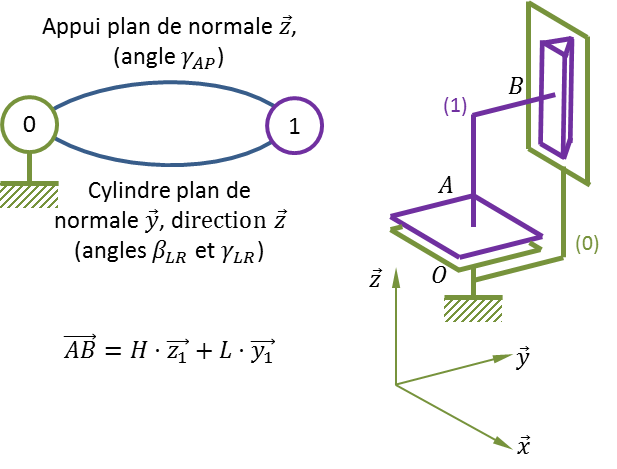
\includegraphics[width=.6\textwidth]{images/chs1}
\end{center}
\end{exemple}

\noindent\colorbox{grisf}{\makebox[\textwidth][l]{%
\textbf{\textsf{Méthode 1 -- Utilisation du torseur cinématique}}
}}

Torseur cinématique de la liaison appui plan en $A$ entre 1 et 0 : 
$\torseurcin{V}{1}{0}_{AP}=\torseurcol{0}{0}{\dot{\gamma}_{10,AP}}{\dot{u}_{10,AP}}{\dot{v}_{10,AP}}{0}{A,\mathcal{R}_1}$

Torseur cinématique de la liaison cylindre -- plan en $B$ puis en $A$ entre 1 et 0 :
$$\torseurcin{V}{1}{0}_{CyP}
=\torseurcol{0}{\dot{\beta}_{10,CyP}}{\dot{\gamma}_{10,CyP}}{\dot{u}_{10,CyP}}{0}{\dot{w}_{10,CyP}}{B,\mathcal{R_1}}
=\torseurcol{0}{\dot{\beta}_{10,CyP}}{\dot{\gamma}_{10,CyP}}{\dot{u}_{10,CyP}+L\cdot\dot{\gamma}_{10,CyP} -H\cdot\dot{\beta}_{10,CyP}}{0}{\dot{w}_{10,CyP}}{B,\mathcal{R}_1}
$$

La liaison équivalente à la chaîne cinématique est donc la suivante : 
$$\{\mathcal{V}_{eq}\}=\torseurcin{V}{1}{0}_{SP}=\torseurcin{V}{1}{0}_{CyP}
=
\torseurcol{0}{0}{\dot{\gamma}_{10,AP}}{\dot{u}_{10,AP}}{\dot{v}_{10,AP}}{0}{A,\mathcal{R}_1}
=\torseurcol{0}{\dot{\beta}_{10,CyP}}{\dot{\gamma}_{10,CyP}}{\dot{u}_{10,CyP}+L\cdot\dot{\gamma}_{10,CyP} -H\cdot\dot{\beta}_{10,CyP}}{0}{\dot{w}_{10,CyP}}{B,\mathcal{R}_1}
$$

D'où :
$$\{\mathcal{V}_{eq}\}
=\torseurcol{0}{0}{\dot{\gamma}_{10,CyP}}{\dot{u}_{10,CyP}+L\cdot\dot{\gamma}_{10,CyP}}{0}{0}{B,\mathcal{R}_1}
\quad
\text{et}
\quad
\left\{
\begin{array}{l}
\dot{u}_{10,APP}=\dot{u}_{10,CyP}+L\cdot\dot{\gamma}_{10,CyP}\\
\dot{\gamma}_{10,APP}=\dot{\gamma}_{10,CyP}
\end{array}
\right.
$$

Cette liaison permet donc deux degrés de liberté : une translations suivant $\vect{x}$ et une rotation autour de $\vect{z}$. Cette liaison équivalente n'est pas associable à une liaison usuelle. 


\noindent\colorbox{grisf}{\makebox[\textwidth][l]{%
\textbf{\textsf{Méthode 2 -- Utilisation du torseur statique}}
}}

Torseur statique de la liaison appui plan en $A$ entre 1 et 0 : 
$\torseurstat{T}{1}{0}_{AP}=\torseurcol{0}{0}{Z_{10,AP}}{L_{10,AP}}{M_{10,AP}}{0}{A,\mathcal{R}_1}$

Torseur statique de la liaison cylindre -- plan en $B$ puis en $A$ entre 1 et 0 :
$$
\torseurstat{T}{1}{0}_{CyP}
=\torseurcol{0}{Y_{10,CyP}}{0}{L_{10,CyP}}{0}{0}{B,\mathcal{R}_1}
=\torseurcol{0}{Y_{10,CyP}}{0}{L_{10,CyP}-HY_{10,CyP}}{0}{0}{B,\mathcal{R}_1}
$$

La liaison équivalente à la chaîne cinématique est donc la suivante : 
$$\{\mathcal{T}_{eq}\}=\torseurstat{T}{1}{0}_{SP}+\torseurstat{T}{1}{0}_{CyP}
\Longleftrightarrow
\left\{
\begin{array}{lll}
X_{eq}&=&0+0\\
Y_{eq}&=&Y_{10,CyP}+0\\
Z_{eq}&=&0+Z_{10,AP}\\
L_{eq}&=&L_{10,AP}\\
&&-HY_{10,CyP}+L_{10,CyP}\\
M_{eq}&=&0+M_{10,AP}\\
N_{eq}&=&0+0\\
\end{array}
\right.
\Longleftrightarrow
\left\{
\begin{array}{l}
X_{eq}=0\\
Y_{eq}=Y_{10,CyP}\\
Z_{eq}=Z_{10,AP}\\
L_{eq}=L_{10,CyP}-HY_{10,CyP}+L_{10,AP}\\
M_{eq}=M_{10,AP}\\
N_{eq}=0\\
\end{array}
\right.
$$

$$
\{\mathcal{T}_{eq}\}=
\torseurcol{0}{Y_{CyP}}{Z_{CyP}}{L_{10,CyP}-HY_{10,CyP}+L_{10,AP}}{M_{10,AP}}{0}{B,\mathcal{R}_1}
$$
Cette liaison permet donc deux degrés de liberté : une translations suivant $\vect{x}$ et une rotation autour de $\vect{z}$. Cette liaison équivalente n'est pas associable à une liaison usuelle. 


\subsubsection*{Interprétation}
On note $\{\mathcal{T}_{ext}\}$ le torseur associé à une action mécanique s'exerçant sur le solide 1. Les composantes de ce torseur sont connues. L'application du PFS au solide donne donc :
$$
\{\mathcal{T}_{ext}\} + \{\mathcal{T}_{eq}\}= \{0\} \Longleftrightarrow
\left\{
\begin{array}{l}
{0}+X_{ext}=0 \\
{Y_{CyP}}+Y_{ext}=0 \\
{Z_{CyP}}+Z_{ext}=0 \\
{L_{10,CyP}-HY_{10,CyP}+L_{10,AP}}+L_{ext}=0 \\
{M_{10,AP}}+M_{ext}=0 \\
{0}+N_{ext}=0 
\end{array}
\right.
$$
Ce système ne permet pas de résoudre les inconnues de liaisons suivantes : $L_{10,CyP}$ et $L_{10,AP}$. En conséquence, le système est hyperstatique d'ordre 1. (Si une des inconnues est donnée, lors peut être déduite).

\textbf{Conséquences du point de vue du calcul des efforts}

\textbf{Si on désire} calculer les inconnues dans les liaisons, il est nécessaire de rendre le système isostatique. Pour cela, il est nécessaire d'avoir $L_{10,CyP}=0$ \textbf{OU} $L_{10,AP}=0$. Dans le premier cas, la liaison cylindre plan est transformée en liaison ponctuelle de normale $\vect{y}$.

Dans le second cas, la liaison appui plan est transformé en liaison linéaire rectiligne "d'axe" $\vect{x}$.

\textbf{Conséquences du point de vue de fonctionnement du mécanisme}

Dans la réalité, les systèmes sont très souvent hyperstatiques ce qui ne les empêche pas de fonctionner. Cela impose cependant des contraintes lors de la fabrication du mécanisme. Ici, le degré d'hyperstatisme provient d'une rotation autour de $\vect{x}$. Il faudrait donc imposer une contrainte angulaire dans le plan $\left(\vect{y},\vect{z}\right)$.

%\subsubsection*{Exemple}
\begin{exemple}

\begin{center}
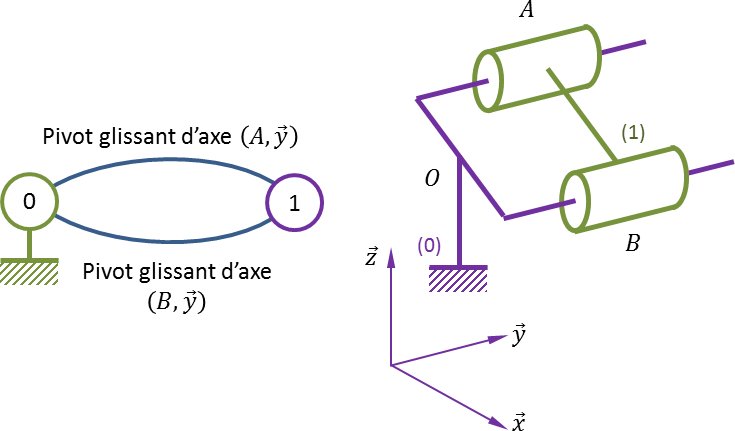
\includegraphics[width=.7\textwidth]{images/chs2}
\end{center}
\end{exemple}

\noindent\colorbox{grisf}{\makebox[\textwidth][l]{%
\textbf{\textsf{Méthode 1 -- Utilisation du torseur cinématique}}
}}
Torseur cinématique de la liaison pivot glissant en $A$ entre 1 et 0 : 
$\torseurcin{V}{1}{0}_{A}=\torseurcol{0}{\dot{\beta}_A}{0}{0}{\dot{v}_A}{0}{A,\mathcal{R}_1}$

Torseur cinématique de la liaison pivot glissant en $B$ puis en $A$ entre 1 et 0 : 
$$\torseurcin{V}{1}{0}_{B}
=\torseurcol{0}{\dot{\beta}_B}{0}{0}{\dot{v}_B}{0}{B,\mathcal{R}_1}
=\torseurcol{0}{\dot{\beta}_B}{0}{0}{\dot{v}_B}{L\dot{\beta}_B}{A,\mathcal{R}_1}
$$


Le torseur équivalent à ces deux liaisons en parallèles se calcule donc ainsi :
$$\{\mathcal{V}_{eq}\}=\torseurcin{V}{1}{0}_{A}=\torseurcin{V}{1}{0}_{B}
\Longleftrightarrow
\left\{
\begin{array}{l}
\dot{\alpha}_{eq}=0=0\\
\dot{\beta}_{eq}=\dot{\beta}_A=\dot{\beta}_B\\
\dot{\gamma}_{eq}=0=0\\
\dot{u}_{eq}=0=0\\
\dot{v}_{eq}=\dot{v}_A=\dot{v}_B\\
\dot{w}_{eq}=0=L\dot{\beta}_B\\
\end{array}
\right.
\Longrightarrow
\torseurcol{0}{0}{0}{0}{\dot{v}_{eq}}{0}{A,\mathcal{R}_1}
$$


\noindent\colorbox{grisf}{\makebox[\textwidth][l]{%
\textbf{\textsf{Méthode 2 -- Utilisation du torseur statique}}
}}

Torseur cinématique de la liaison pivot glissant en $A$ entre 1 et 0 : 
$\torseurstat{T}{0}{1}_{A}=\torseurcol{X_A}{0}{Z_A}{L_A}{0}{N_A}{A,\mathcal{R}_1}$

Torseur cinématique de la liaison pivot glissant en $B$ puis en $A$ entre 1 et 0 : 
$$\torseurstat{T}{0}{1}_{B}
=\torseurcol{X_B}{0}{Z_B}{L_B}{0}{N_B}{B,\mathcal{R}_1}
=\torseurcol{X_B}{0}{Z_B}{L_B}{-LZ_B}{N_B}{A,\mathcal{R}_1}
$$

Le torseur équivalent est donc :
$$
\{ T_{eq}\}=\torseurstat{T}{0}{1}_{A}+\torseurstat{T}{0}{1}_{B} 
\Longleftrightarrow
\left\{
\begin{array}{l}
X_{eq}=X_A+X_B\\
Y_{eq}=0\\
Z_{eq}=Z_A+Z_B\\
L_{eq}=L_A+L_B\\
M_{eq}=-LZ_B\\
N_{eq}=N_A+N_B\\
\end{array}
\right.
\Longrightarrow
\{ T_{eq}\}=\torseurcol{X_A+X_B}{0}{Z_A+Z_B}{L_A+L_B}{-LZ_B}{N_A+N_B}{A,\mathcal{R}_1}
$$


\subsection*{Interprétation}

On note $\{\mathcal{T}_{ext}\}$ le torseur associé à une action mécanique s'exerçant sur le solide 1. Les composantes de ce torseur sont connues. L'application du PFS au solide donne donc :
$$
\{\mathcal{T}_{ext}\} + \{\mathcal{T}_{eq}\}= \{0\} \Longleftrightarrow
\left\{
\begin{array}{l}
X_A+X_B+X_{ext}=0 \\
0+Y_{ext}=0 \\
Z_A+Z_B+Z_{ext}=0 \\
L_A+L_B+L_{ext}=0 \\
-LZ_B+M_{ext}=0 \\
N_A+N_B+N_{ext}=0 
\end{array}
\right.
$$
Ce système ne permet pas de résoudre les inconnues de liaisons suivantes : $X_A$, $X_B$, $L_A$, $L_B$, $N_A$, $N_B$. Attention, la 5\ieme{} équation permet de calculer $Z_B$ et le 4\ieme{} de calculer $Z_A$. 

Ici, le système est hyperstatique d'ordre 3.

\textbf{Conséquences du point de vue du calcul des efforts}

\textbf{Si on désire} calculer les inconnues dans les liaisons, il existe plusieurs combinaisons 
de composantes à rendre nulles pour rendre le système isostatique. 

Par exemple, si $X_A$, $L_A$ et $N_A$ sont nuls, la liaison en A est transformée en une liaison ponctuelle de normale A. 


\textbf{Conséquences du point de vue de fonctionnement du mécanisme}

Ici, le degré d'hyperstatisme provenant de deux rotations autour de $\vect{x}$ et autour de $\vect{z}$, ainsi que d'un effort suivant $\vect{x}$, il faudrait donc 3 conditions géométriques : 
\begin{itemize}
\item une distance suivant $\vect{x}$ (entraxe);
\item le parallélisme dans le plan $(\vect{x},\vect{y})$;
\item le parallélisme dans le plan $(\vect{y},\vect{z})$.
\end{itemize}


%\subsubsection*{Exemple}

%\begin{center}
%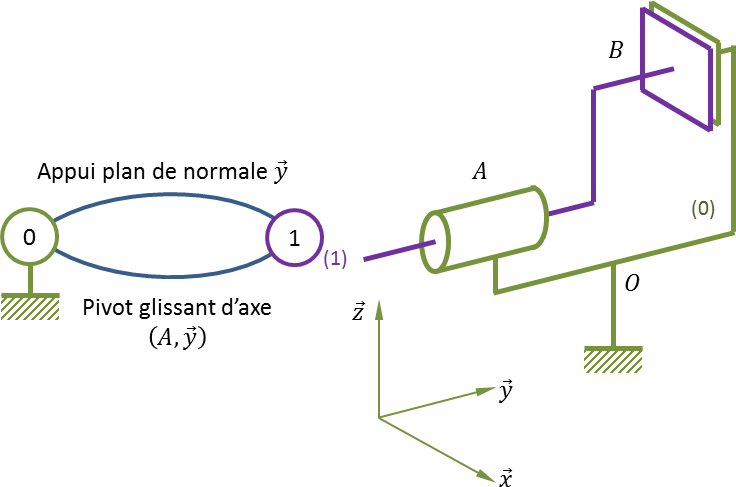
\includegraphics[width=.7\textwidth]{images/chs3}
%\end{center}

%\noindent\colorbox{grisf}{\makebox[\textwidth][l]{%
%\textbf{\textsf{Méthode 1 -- Décomposition du torseur cinématique}}
%}}


%\noindent\colorbox{grisf}{\makebox[\textwidth][l]{%
%\textbf{\textsf{Méthode 2 -- Utilisation du PFS}}
%}}



\subsection{Notion de mobilités dans les chaînes fermées}
\begin{warn}
\textbf{Ce vocabulaire est utilisé dans le cas des chaînes fermées. Dans ce cas, il est alors possible d'écrire des lois entrées sorties.}
\end{warn}

\subsubsection{Cas des mobilités utiles}

\begin{defi}

Les mobilités dites "utiles" permettent à un mécanisme de transformer et de transmettre un mouvement. L'écriture de la loi \textbf{entrée -- sortie} permet d'ajouter une équation cinématique et donc, le cas échéant, d'identifier une inconnue supplémentaire. 

\end{defi}

\begin{methode}
L'écriture de la fermeture de chaîne cinématique permet telle qu'on l'a vu ultérieurement permet d'obtenir la loi entrée -- sortie d'un mécanisme.

Une seconde solution pour obtenir la loi entrée sortie d'un mécanisme et d'utiliser la composition du torseur cinématique.
\end{methode}



\begin{exemple}

\textit{Modélisation de la pompe du pilote automatique de voilier}

\noindent\begin{minipage}[c]{.45\linewidth}
\begin{center}
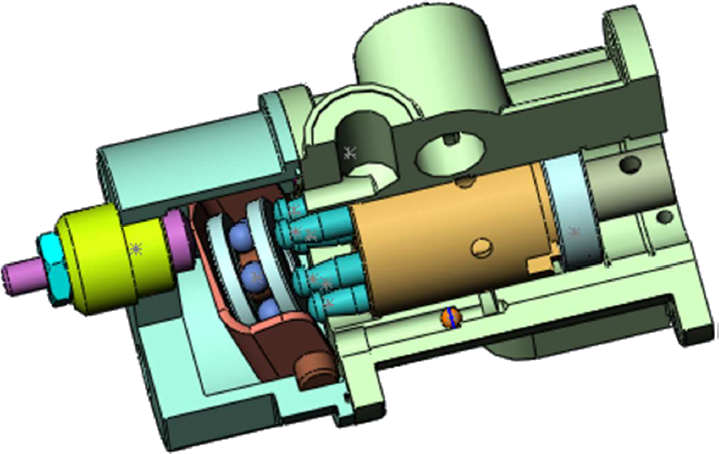
\includegraphics[width=.9\textwidth]{images/pompe1}
\end{center}
\end{minipage}\hfill
\begin{minipage}[c]{.45\linewidth}
\begin{center}
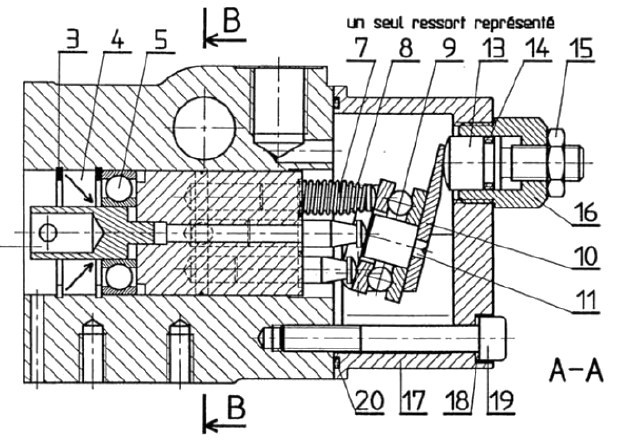
\includegraphics[width=.9\textwidth]{images/pompe2}
\end{center}
\end{minipage}

\noindent\begin{minipage}[c]{.55\linewidth}
\begin{center}
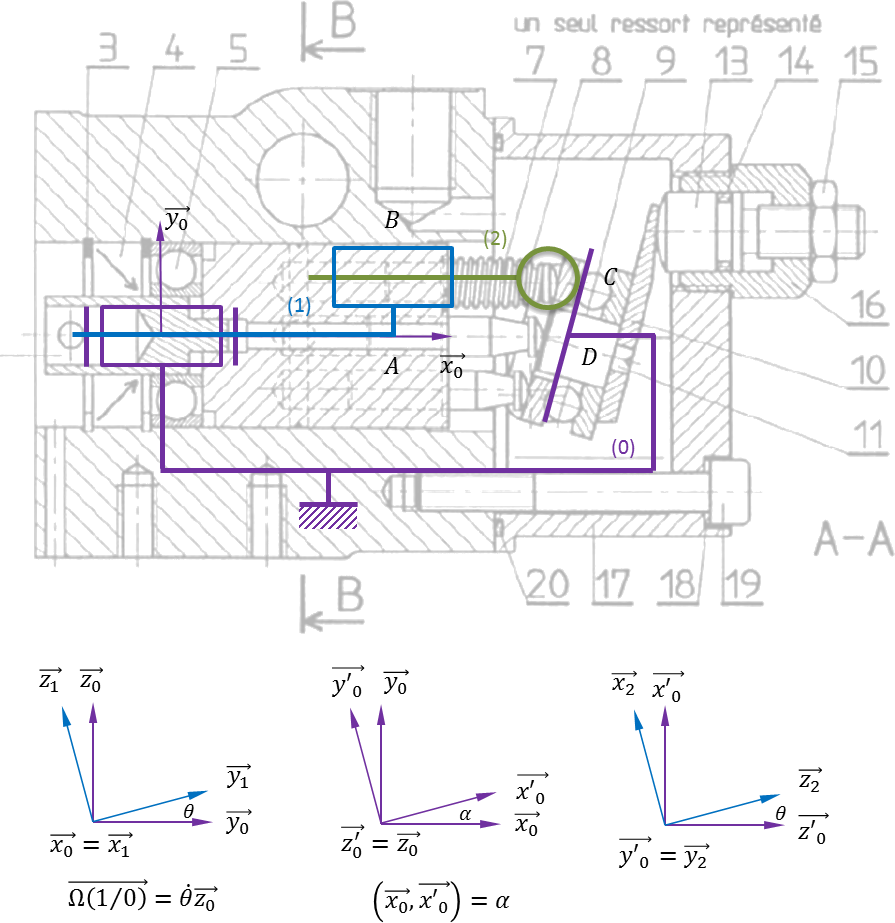
\includegraphics[width=.9\textwidth]{images/pompe3}
\end{center}
\end{minipage}\hfill
\begin{minipage}[c]{.4\linewidth}
\begin{center}
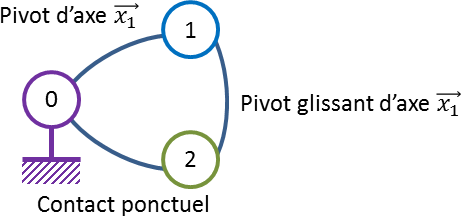
\includegraphics[width=.95\textwidth]{images/pompe4}
\end{center}
\end{minipage}

On cherche à obtenir une relation entre la vitesse de rotation de l'ensemble 1 ($\dot{\theta}$) en fonction de la vitesse de translation d'un piston $\dot{\lambda(t)}$. 

$\lambda$ est défini tel que lorsque $\alpha=\dfrac{\pi}{2}$, $\lambda=0$. Dans ces conditions, $C$ et $D$ sont alignés suivant le vecteur $\vect{y_1}$. On a alors $\vect{BC} =\left( L+\lambda(t)\right) \vect{x_0}$ et $\vect{AD}=L\vect{x_0}$.

\textbf{Fermeture de chaîne géométrique $ABCD$ :}


On a donc : 
\begin{eqnarray*}
\vect{AB}+\vect{BC}+\vect{CD}+\vect{DA}=\vect{0} \\
R\vect{y_1}+\left(L+\lambda(t)\right) \vect{x_0}-r\vect{z_2}-L\vect{x_0}=\vect{0}\\
R\vect{y_1}+ \lambda(t) \vect{x_0} - r\vect{x_2}=\vect{0} \\
R\left(\cos\theta\vect{y_0}+\sin\theta\vect{z_0} \right)+ \lambda(t) \vect{x_0} - r\left(\cos\theta\vect{x'_0}-\sin\theta\vect{z'_0} \right)
=\vect{0} \\
R\left(\cos\theta\vect{y_0}+\sin\theta\vect{z_0} \right)+ \lambda(t) \vect{x_0} - r\left(\cos\theta\left(\cos\alpha\vect{x_0}+\sin\alpha\vect{y_0} \right)-\sin\theta\vect{z_0}\right)
=\vect{0} \\
\end{eqnarray*}

Par ailleurs, $r= \dfrac{R}{\sin\alpha}  $, en conséquence : 
$$
\left(\lambda(t) -\dfrac{R}{\sin\alpha}\cos\theta\cos\alpha\right) \vect{x_0}
+\left(R\cos\theta -\dfrac{R}{\sin\alpha}\cos\theta\sin\alpha\right) \vect{y_0}
+\left(R\sin\theta + \dfrac{R}{\sin\alpha}\sin\theta\right) \vect{z_0}
=\vect{0} 
$$

En projection l'équation sur $\vect{x_0}$, $\vect{y_0}$ et $\vect{z_0}$ :

\begin{eqnarray*}
\text{Projection sur }\vect{x_0} : \quad  
\lambda(t) -\dfrac{R}{\sin\alpha}\cos\theta\cos\alpha = 0 \\
\text{Projection sur }\vect{y_0} : \quad  
R\cos\theta -R\cos\theta= 0  \\
\text{Projection sur }\vect{z_0} : \quad  
R\sin\theta + \dfrac{R}{\sin\alpha}\sin\theta = 0
\end{eqnarray*}

La projection sur $\vect{x}$ donne directement une relation entre $\lambda (t)$ et $\theta$. En dérivant cette expression on a :
$$
\dot{\lambda} (t)- R \cdot \dfrac{\cos\alpha}{\sin\alpha} \cdot  \dot{\theta }\sin \theta= 0
$$


\textbf{Composition du torseur cinématique :}

$$
\torseurcin{V}{1}{0}=
\torseurl{
\vecto{1}{0}=\dot{\theta}\vect{x_0}
}{
\vectv{A}{1}{0}=\vect{0}
}{
A
}
=
\torseurl{
\vecto{1}{0}=\dot{\theta}\vect{x_0}
}{
\vectv{D}{1}{0}=\vect{0}
}{
D
}
$$

$$
\torseurcin{V}{2}{1}=
\torseurl{
\vecto{2}{1}=\dot{\beta}\vect{x_0}
}{
\vectv{B}{2}{1}=\dot{\lambda}\vect{x_0}
}{
B
}
=
\torseurl{
\vecto{2}{1}=\dot{\beta}\vect{x_0}
}{
\begin{array}{ll}
\vectv{D}{2}{1}
&=\dot{\lambda}\vect{x_0}+ \vect{DB}\wedge \vecto{2}{1}\\
&=\dot{\lambda}\vect{x_0}+ \left(-L\vect{x_0}+R\vect{y_1} \right)\wedge \vecto{2}{1}\\
&=\dot{\lambda}\vect{x_0}+ \left(-L\vect{x_0}+R\vect{y_1} \right)\wedge \dot{\beta}\vect{x_0}\\
%&=\dot{\lambda}\vect{x_0}-R\dot{\beta}\vect{z_1}\\
&=\dot{\lambda}\vect{x_0}-R\dot{\beta}\vect{z_1}\\
&=\dot{\lambda}\vect{x_0}-R\dot{\beta}\left( \cos\theta\vect{z_0}-\sin\theta\vect{y_0}\right)%\\
%&=\dot{\lambda}\left(\cos\alpha\vect{x'_0}- \sin\alpha\vect{y'_0}\right)
%-R\dot{\beta}\left( \cos\theta\vect{z_0}-\sin\theta\vect{y_0}\right)%\\
%&=\dot{\lambda}\left(\cos\alpha\vect{x'_0}- \sin\alpha\vect{y'_0}\right)
%\\
%&-R\dot{\beta}\left( \cos\theta\vect{z'_0}-\sin\theta\left(\cos\alpha\vect{y'_0}+\sin\alpha\vect{x'_0} \right)\right)
\end{array}
}{
A
}
$$


$$
\torseurcin{V}{2}{0}=
\torseurcin{V}{2}{1}+\torseurcin{V}{1}{0}=
\torseurl{
\vecto{2}{0}=\vecto{2}{1}+\vecto{1}{0}
}{
\vectv{D}{2}{0}=\vectv{D}{2}{1}+\vectv{D}{1}{0}
}{
D
}
$$

$$
\torseurcin{V}{2}{0}=
\torseurcin{V}{2}{1}+\torseurcin{V}{1}{0}=
\torseurl{
\begin{array}{ll}
\vecto{2}{0}=\dot{\beta}\vect{x_0}+\dot{\theta}\vect{x_0}
\end{array}
}{
\begin{array}{lll}
\vectv{A}{2}{0}
&=&\dot{\lambda}\vect{x_0}-R\dot{\beta}\vect{z_1} \\
%&=&\dot{\lambda}\vect{x_0}-R\dot{\beta}\vect{z_1} \\
\end{array}
}{
A
}
$$

Par ailleurs la liaison entre 2 et 0 est une liaison ponctuelle de normale $\vect{y'_0}$ :
$$
\torseurcin{V}{2}{0}=\torseurl{
\vecto{2}{0}=\dot{\psi}\vect{x'_0}+\dot{\theta}\vect{y'_0}+\dot{\varphi}\vect{z'_0}
}{
\begin{array}{lll}
\vectv{D}{2}{0}&=&\left[\dfrac{-r\vect{x_2}}{dt}\right]_{\mathcal{R}_0}\\
&=&r\dot{\theta}\vect{z_2} \\
&=&r\dot{\theta}\left( \cos\theta\vect{z'_0}+\sin\theta\vect{x'_0} \right) \\
&=&r\dot{\theta}\left( \cos\theta\vect{z_0}+\sin\theta\left( \cos\alpha\vect{x_0}
+\sin\alpha\vect{y_0} \right) \right) 
\end{array}
}{D}
$$


En identifiant les torseurs (et avec $r= \dfrac{R}{\sin\alpha} $), la projection sur $\vect{y'_0}$ on a donc : 
$$
\dot{\lambda} = \dfrac{R}{\sin\alpha}\dot{\theta} \sin\theta \cos\alpha
$$


%On a donc nécessairement : $\vectv{A}{2}{0}\cdot\vect{y'_0}=\vect{0}$.
%$$
%-\dot{\lambda}\sin\alpha-r\dot{\beta}\sin\theta\cos\alpha=0
%\quad \Longleftrightarrow \quad 
%\dot{\lambda}\sin\alpha = r\dot{\beta}\sin\theta\cos\alpha
%\quad \Longleftrightarrow \quad 
%\dot{\lambda}\tan\alpha = r\dot{\beta}\sin\theta
%$$

%$$
%=
%\torseurl{
%\vecto{2}{0}=\dot{\psi_1}\vect{x'_1}
%+\dot{\psi_2}\vect{y'_1}
%+\dot{\psi_3}\vect{z'_1}
%}{
%\begin{array}{ll}
%\vectv{A}{2}{0}
%&=\dot{\mu}_1 \vect{y'_0} + \dot{\mu}_2 \vect{z'_0} + \vect{AC}\wedge \vecto{2}{0}\\
%&=\dot{\mu}_1 \vect{y'_0} + \dot{\mu}_2 \vect{z'_0} 
%+ \left( \dot{\psi_1}\vect{x'_1} + \dot{\psi_2}\vect{y'_1} + \dot{\psi_3}\vect{z'_1}\right) \wedge \left( l\vect{x_0}+R\vect{y'_1}\right)\\
%& = 
%\dot{\mu}_1 \vect{y'_0} + \dot{\mu}_2 \vect{z'_0} 
%+\dot{\psi_1}l \sin\alpha\vect{z_0}
%+\dot{\psi_2}l \vect{y'_1}\wedge \vect{x_0}
%+\dot{\psi_3}l \vect{z'_1}\wedge \vect{x_0}
%+\dot{\psi_1}R \vect{z'_1}
%-\dot{\psi_3}R \vect{x'_1}
%\\
%\end{array}
%}{
%A
%}
%$$


%\begin{eqnarray*}
%\torseurcin{V}{0}{1} + \torseurcin{V}{1}{2} + \torseurcin{V}{2}{0} = \{0\} \Longleftrightarrow
%\torseurl{
%\vecto{0}{1}+\vecto{1}{2}+\vecto{2}{0}=\vect{0}
%}{
%\vectv{A}{0}{1}+\vectv{A}{1}{2}+\vectv{A}{2}{0}=\vect{0}
%}{
%A
%}\\
%\torseurl{
%\dot{\theta}\vect{x_0}
%+\dot{\beta}\vect{x_0}
%+\dot{\psi_1}\vect{x_0}
%+\dot{\psi_2}\vect{y_0}
%+\dot{\psi_3}\vect{z_0}
%=\vect{0}
%}{
%\vect{0}
%+\left( \dot{\lambda} \vect{x_0} + \vect{AB}\wedge \vecto{1}{2}\right)
%+\left( \dot{\mu}_1 \vect{y'_0} + \dot{\mu}_2 \vect{z'_0} + \vect{AC}\wedge \vecto{2}{0}\right)
%=\vect{0}
%}{
%A
%}
%\end{eqnarray*}

\end{exemple}
\subsubsection{Cas des mobilités internes}

\begin{defi}
\textbf{Mobilité interne}

Il s'agit du nombre de paramètres indépendants à imposer pour connaître les mouvements (ou positions) des pièces internes seulement du mécanisme (indépendamment de la loi entrée sortie). 

\end{defi}

\begin{exemple}
\textit{Pompe}

Sur la pompe précédente on peut observer que le piston 2 est en liaison pivot glissant avec la pièce 1. On observe que la rotation propre du piston ne change rien au fonctionnement du mécanisme. Ainsi, dans le cas où cette rotation était supprimé, le fonctionnement serait inchangé. 

La rotation de ce piston pourrait donc être supprimée et la liaison pivot glissant pourrait être remplacée par une liaison glissière. 
\end{exemple}

%\subsection{Définitions}

\section{Notion de puissance délivrée par un mécanisme}

\begin{defi}
\textbf{Puissance}

La puissance dans un mécanisme est donnée par le co-moment du torseur statique et du torseur cinématique. Elle s'exprime en Watt :

$$
\mathcal{P}=
\torseurstat{T}{\overline{E}}{E}\otimes\torseurcin{V}{\overline{E}}{E}
$$
$$
\mathcal{P}=
\torseurcol{X}{Y}{Z}{L}{M}{N}{A,\mathcal{R}} \otimes 
\torseurcol{\alpha}{\beta}{\gamma}{u}{v}{w}{A,\mathcal{R}}
=
\torseurl{\vectf{\overline{E}}{E}}{\vectm{A}{\overline{E}}{E}}{A,\mathcal{R}}
\otimes
\torseurl{\vecto{\overline{E}}{E}}{\vectv{A}{\overline{E}}{E}}{A,\mathcal{R}}
$$
$$
\mathcal{P}=\vectf{\overline{E}}{E}\cdot\vectv{A}{\overline{E}}{E}
+\vecto{\overline{E}}{E}\cdot\vectm{A}{\overline{E}}{E}
$$
\end{defi}

\begin{exemple}
\textit{Puissance consommée par une liaison pivot sans frottement :}
$$
\mathcal{P}=
\torseurcol{X}{Y}{Z}{L}{M}{0}{A,\mathcal{R}} \otimes 
\torseurcol{0}{0}{\dot{\gamma}}{0}{0}{0}{A,\mathcal{R}}
=
\left[\begin{array}{c}
X\\Y\\Z
\end{array}
\right]
\cdot
\left[\begin{array}{c}
0\\0\\0
\end{array}
\right]
+
\left[\begin{array}{c}
0\\0\\ \dot{\gamma}
\end{array}
\right]
\cdot
\left[\begin{array}{c}
L \\ M \\0
\end{array}
\right]
=0
$$

Dans les liaisons sans frottement la puissance dissipée est nulle. 


\textit{Puissance consommée par une liaison pivot avec frottement visqueux:}

Le couple de frottement visqueux est proportionnel à la vitesse de rotation : $C_f=f\dot{\gamma}$
$$
\mathcal{P}=
\torseurcol{X}{Y}{Z}{L}{M}{f\dot{\gamma}}{A,\mathcal{R}} \otimes 
\torseurcol{0}{0}{\dot{\gamma}}{0}{0}{0}{A,\mathcal{R}}
=
\left[\begin{array}{c}
X\\Y\\Z
\end{array}
\right]
\cdot
\left[\begin{array}{c}
0\\0\\0
\end{array}
\right]
+
\left[\begin{array}{c}
0\\0\\ \dot{\gamma}
\end{array}
\right]
\cdot
\left[\begin{array}{c}
L \\ M \\ f\dot{\gamma}
\end{array}
\right]
=f\dot{\gamma}^2
$$

\textit{Puissance de coupe}


\end{exemple}

\begin{thebibliography}{2}
\bibitem{mc}{Mécanique -- Partie 5, Analyse des mécanismes : chaînes de solides. Cours de Maryline Carrez -- PT (2009--2010). Lycée Jules Haag, Besançon.}
\end{thebibliography}



\end{document}

